%%%%%%%%%%%%%%%%%%%%%%%%%%%%%%%%%%%%%%%%%%%%%%%%%%%%%%%%%%%%%%%%%%%%%%%%%%%%%%%%
%2345678901234567890123456789012345678901234567890123456789012345678901234567890
%        1         2         3         4         5         6         7         8


%\documentclass[a4paper, 12pt, twocolumn]{article}   
\documentclass[a4paper, 12pt]{article}   

% The following packages can be found on http:\\www.ctan.org
\usepackage{graphicx}% for pdf, bitmapped graphics files
\usepackage{graphbox}
\usepackage{bm}
\usepackage[english]{babel}
\pagenumbering{arabic}
\usepackage[a4paper,top=2.5cm,bottom=2.5cm,left=2cm,right=2cm,marginparwidth=1.75cm]{geometry}
\newcommand{\uvec}[1]{\boldsymbol{\hat{\textbf{#1}}}}
\usepackage[table,xcdraw]{xcolor}
\usepackage[utf8x]{inputenc}
\usepackage{amsmath}
\usepackage{url}
\usepackage{longtable}
\usepackage[font={footnotesize}]{caption}
\usepackage[labelfont=bf]{caption}
\usepackage{subfig}
\usepackage[colorinlistoftodos]{todonotes}
\usepackage{cite}
\usepackage{indentfirst}
\usepackage{color}
\usepackage{pdflscape}
\usepackage{multicol}
\usepackage{float}
\usepackage{supertabular}
\usepackage{subfig}
\usepackage{booktabs}
\usepackage{verbatim}
\usepackage{amssymb}
\usepackage{multirow}
\renewcommand{\baselinestretch}{1}
%\setlength{\baselineskip}{0.5cm}

\begin{document}
\begin{titlepage}
\newcommand{\HRule}{\rule{\linewidth}{0.5mm}} % Defines a new command for the horizontal lines, change thickness here

\center % Center everything on the page
 
%----------------------------------------------------------------------------------------
% HEADING SECTIONS
%----------------------------------------------------------------------------------------

%\textsc{\LARGE EPFL}\\[1.5cm] % Name of your university/college

%----------------------------------------------------------------------------------------
% LOGO SECTION
%----------------------------------------------------------------------------------------

\includegraphics[scale=1]{EPFL-Logo.jpg}\\[2cm] % Include a department/university logo - this will require the graphicx package
 
%----------------------------------------------------------------------------------------

\textsc{\Large Applied Biostatistics \hspace{4pt} -\hspace{6pt} MATH-493}\\[1cm] % Major heading such as course name
%\textsc{\large sous-titre}\\[0.5cm] % Minor heading such as course title

%----------------------------------------------------------------------------------------
% TITLE SECTION
%----------------------------------------------------------------------------------------

\HRule \\[0.4cm]
{ \LARGE \bfseries Assignment 3: \\ Generalized Linear Models in R,\vspace{6pt}\\ Horseshoe Crab Dataset}\\[0.4cm] % Title of your document
\HRule \\[1cm]
 
%----------------------------------------------------------------------------------------
% AUTHOR SECTION
%----------------------------------------------------------------------------------------

\Large \emph{Authors:}\\[0.5cm]
\textsc{Wong Wen Yan},   \\[2cm] % Your name
\Large \emph{Professor:}\\[0.5cm]
Darlene \textsc{Goldstein}  \\[3cm]



%----------------------------------------------------------------------------------------
% DATE SECTION
%----------------------------------------------------------------------------------------

{\large \today}\\[1cm] % Date, change the \today to a set date if you want to be precise



\vfill % Fill the rest of the page with whitespace

\end{titlepage}



\thispagestyle{plain}
\pagestyle{plain}


%%%%%%%%%%%%%%%%%%%%%%%%%%%%%%%%%%%%%%%%%%%%%%%%%%%%%%%%%%%%%%%%%%%%%

%%%% EXAMPLE OF FIGURE %%%%

% \begin{figure}[h]
% \centering
% \includegraphics[width=0.75\textwidth]{EXAMPLE1.png}
% \caption{\label{fig:skin}\textbf{A schematic of the skin's structure\cite{figureskin}.}} \end{figure}

%%%% EXAMPLE OF MULTIFIGURE %%%%

% \begin{figure}[h]
% \centering
% \subfloat[\label{fig:bioprint}]{\includegraphics[align=c,scale=0.5]{bioprint.png}} \hspace{20px} 
% \subfloat[\label{fig:porous}]{\includegraphics[align=c,scale=1]{porous.jpg}} \hspace{20px} 
% \subfloat[\label{fig:plant}]{\includegraphics[align=c,scale=1]{plant.jpg}} 
% \caption{\label{fig:vascularization} \textbf{Different methods to improve vascularization (a)} Schematic diagrams and fluorescent micrographs of bioprinted tubes which could be used as vessels \textbf{(b)} SEM micrograph of a 65NaCl-PGS porous scaffold \textbf{(c)} Fluorescent microspheres (red) perfused in a decellularized spinach leaf.}
% \end{figure}

%%%% TO CITE %%%%

% go to google scholar, look for your paper, click on cite (or the '') then click on BibTex, then copy paste this on the references.bib file. You can change the name of the paper by whatever you want, see example
%\cite{NAMEOFTHEPAPER}

%%%%%%%%%%%%%%%%%%%%%%%%%%%%%%%%%%%%%%%%%%%%%%%%%%%%%%%%%%%%%%%%%%%%%

%Table des matières
\tableofcontents
\thispagestyle{empty} % Page count starts next page
\newpage 

\pagenumbering{arabic} 

\section{Introduction}
\noindent The dataset chosen for this study is the Horseshoe Crab dataset. The goal of this study is to predict the number of spines present in a horseshoe crab, given 5 independent variables: 

\begin{enumerate}
  \item \texttt{y}: whether the female crab has a satellite (\texttt{1} = yes, \texttt{0} = no), binary
  \item \texttt{weight}: weight in grams, real valued and positive
  \item \texttt{color}: color of horseshoe crab, can take on four possible values (1, 2, 3, 4), categorical
  \item \texttt{width}: width of the female crab in centimeters, real valued and positive
  \item \texttt{sat}: number of satellites (\texttt{y} = 0 if and only if \texttt{sat} = 0), positive integer
\end{enumerate}

\noindent The dependent variable \texttt{spine} is discrete and can only take on positive values. In particular, \texttt{spine} only has three possible values: 1, 2 and 3. Since the dependent variable is a count variable, a linear regression model, which has the form 


$$ Y = \beta^TX \,+ \epsilon \, , \quad \epsilon \sim \mathcal{N}(0,\,\sigma^{2})\ $$
$$ \beta, X \in \mathbb{R}^n $$

\noindent will not be able to represent the discrete and non-negative nature of \texttt{spine} because $\epsilon$ is a continuous random variable which can take values from $-\infty$ to $+\infty$. To model a count variable, we need to consider generalized linear models with discrete and non-negative distribution functions (eg. Poisson distribution, Negative Binomial distribution). In other words, the model must fulfill
\begin{equation}
    f_Y(y) =
    \begin{cases}
      \exp(a(y)b(\theta) + c(\theta) + d(y)), & \text{if}\ y \in \mathbb{Z^+} \\
      0, & \text{otherwise}
    \end{cases}
    \label{discrete-exponential-family}
\end{equation}
$$ \eta(E(Y|X)) = \beta^TX $$
where $\eta$ is the link function, and $ \beta, X \in \mathbb{R}^n $. \\
\indent In this study, three instances of such generalized linear models will be used to predict \texttt{spine}, namely: \textbf{\textit{Poisson regression model}}, \textbf{\textit{Quasi Poisson regression model}}, and \textbf{\textit{Negative Binomial regression model}}. The best models of each type will be compared against each other using multiple metrics and criteria. Finally, the best model will be selected.     

\section{Initial Data Analysis}
Before fitting models to the data, exploratory data analysis was carried to gain better understanding of the structure of the dataset, using common visualization tools presented below. These visualizations also help to reveal the relative importance of the independent variables in predicting \texttt{spine}.

\subsection{Overview of dataset}
\begin{figure}[H]
\begin{center}
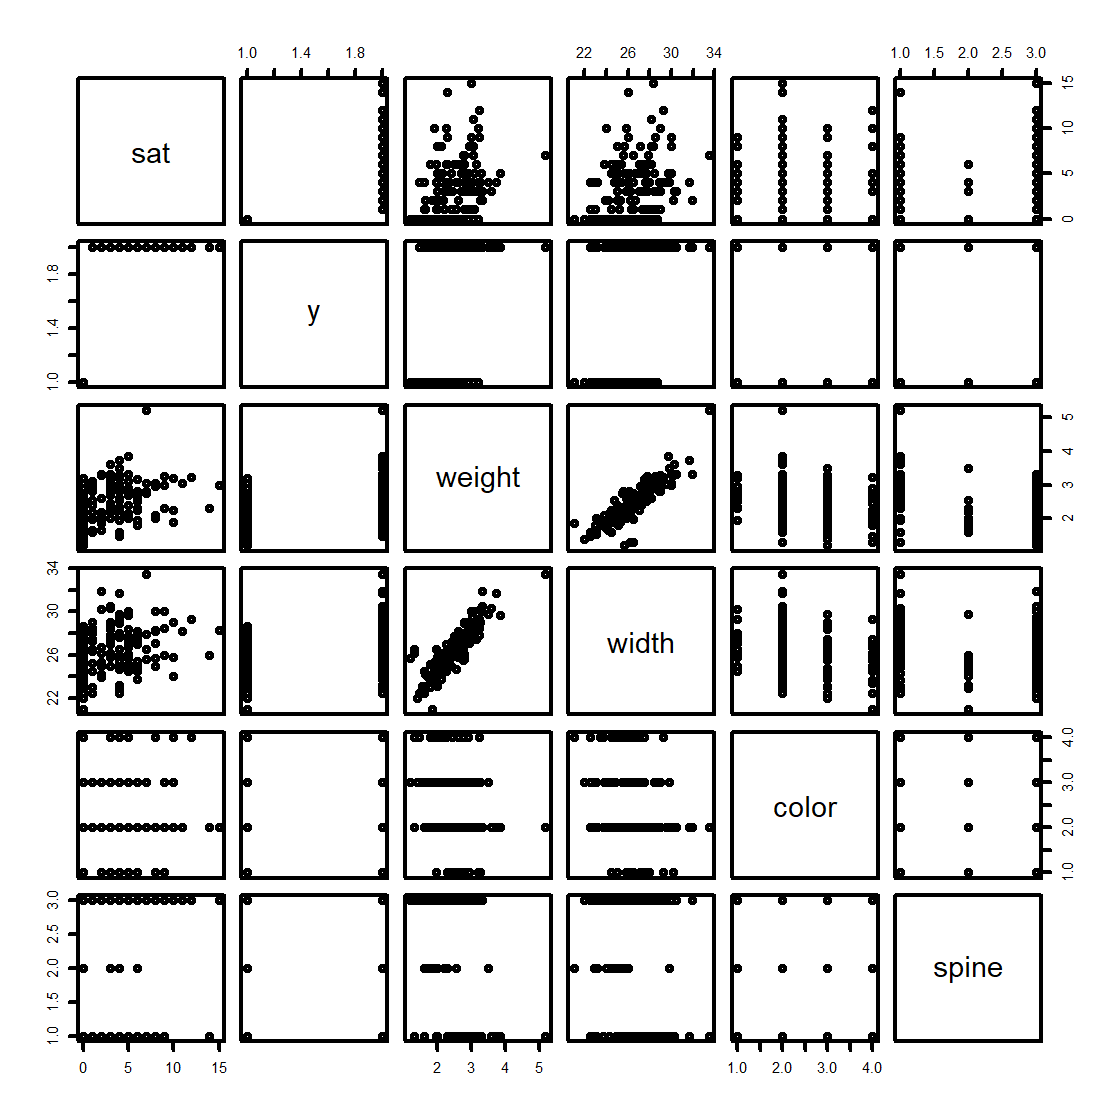
\includegraphics[scale=1.4]{initial-data-analysis/scatter-matrix}
\caption{Scatter matrix of the Horseshoe Crab dataset. Key observations: (a) \texttt{spine}, \texttt{color}, \texttt{y} and \texttt{sat} are indeed discrete valued. (b) No noticeable strong correlation between \texttt{spine} and any one of the independent variables. (c) Strong correlation between \texttt{weight} and \texttt{width}, this may cause multicollinearity issues in modeling if both variables are included.}
\label{scatter-matrix}
\end{center}
\end{figure}

\subsection{Importance of numeric predictors}

\begin{table}[H]
\centering
\begin{tabular}{rrrrr}
  \hline
 & sat & weight & width & spine \\ 
  \hline
sat & 1.00 & 0.37 & 0.34 & -0.09 \\ 
  weight & 0.37 & 1.00 & 0.89 & -0.17 \\ 
  width & 0.34 & 0.89 & 1.00 & -0.12 \\ 
  spine & -0.09 & -0.17 & -0.12 & 1.00 \\ 
   \hline
\end{tabular}
\caption*{\textbf{Table 1:} Correlation Matrix between numeric predictors and \texttt{spine}. Since \texttt{y} and \texttt{color} are categorical, their numerical correlation with \texttt{spine} is not meaningful for interpretation. Key observations: (a) No significant linear dependence between \texttt{spine} and any of the \texttt{spine} and any of the numeric predictors. Numeric predictors might be less useful. (b) Strong positive correlation between \texttt{weight} and \texttt{width} (0.89), this will very likely cause multicollinearity issues.}
\label{tab:correlation-matrix}
\end{table}

\begin{figure}
    \centering
    \subfloat[Distribution of \texttt{spine} w.r.t \texttt{weight}]{{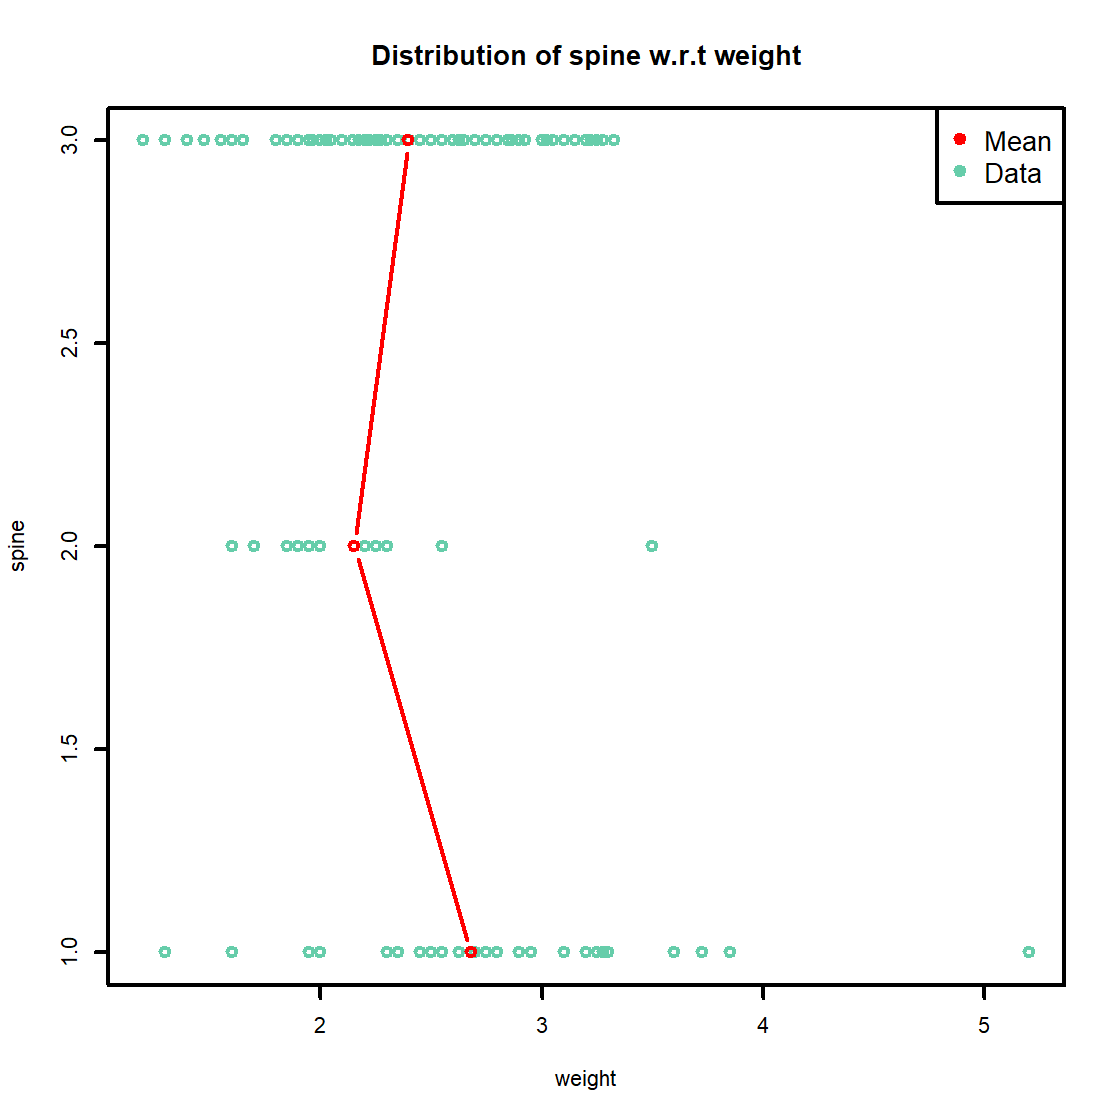
\includegraphics[scale=1.0]{initial-data-analysis/distribution-of-spine-wrt-weight} }}
    \qquad
    \subfloat[Distribution of \texttt{spine} w.r.t \texttt{sat}]{{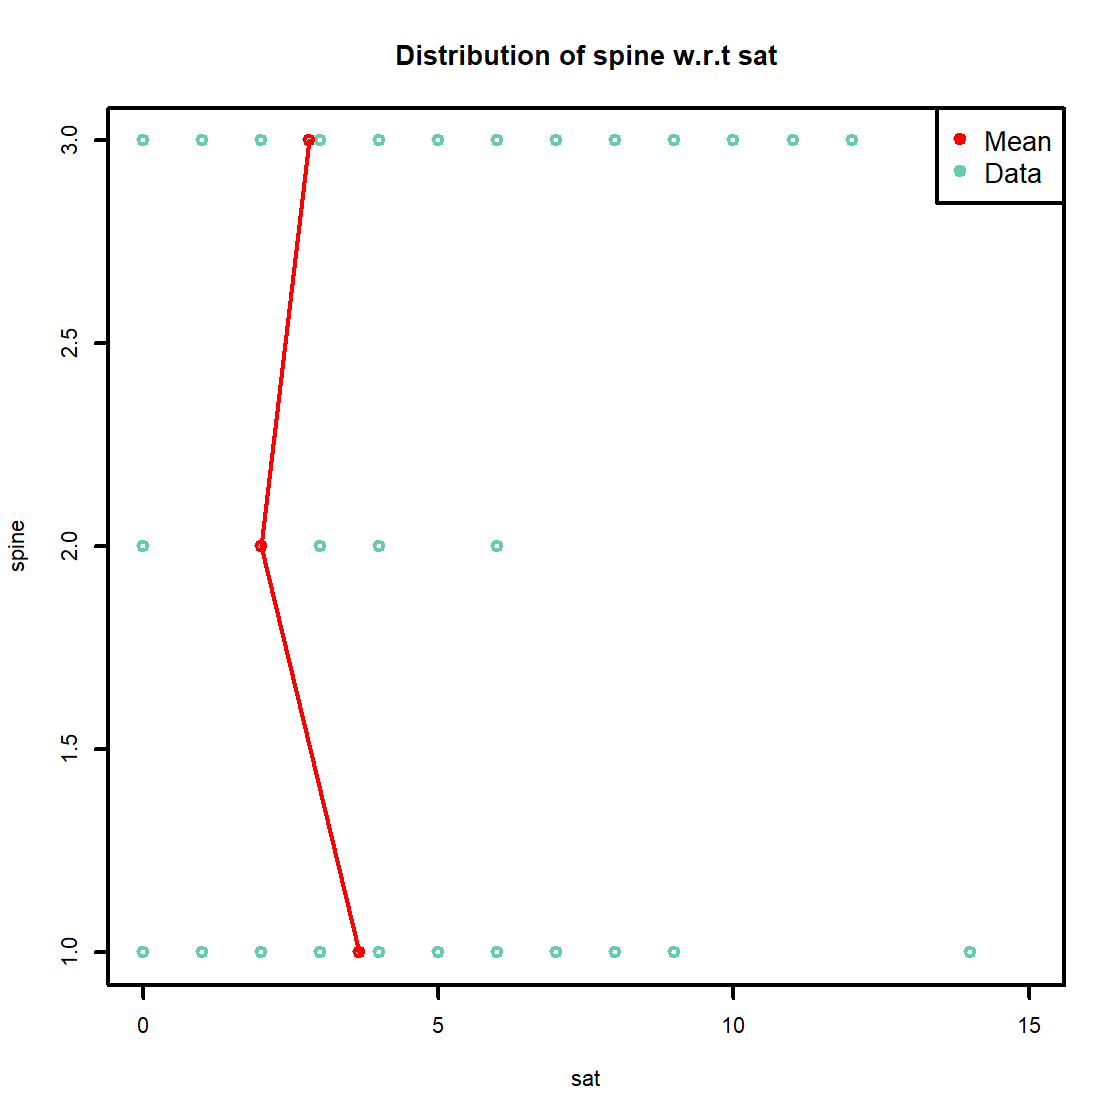
\includegraphics[scale=1.0]{initial-data-analysis/distribution-of-spine-wrt-sat} }}
    \caption{Red points indicate the mean of predictor when \texttt{spine} is fixed at a certain value. If we split the dataset into three classes based on the value of \texttt{spine}, it is clear that the intra-class variances of \texttt{weight} and \texttt{sat} are very large. On top of that, the differences in inter-class means of \texttt{weight} and \texttt{sat} are relatively small. We can expect \texttt{weight} and \texttt{sat} themselves be less useful in predicting \texttt{spine}. Besides, the distribution of \texttt{spine} w.r.t \texttt{width} is not displayed here, but it is expected to behave in a similar fashion as \texttt{weight} since they are highly correlated.}
    \label{distribution-of-spine-wrt-weight-sat}
\end{figure}




\subsection{Importance of categorical predictors}
\begin{figure}[H]
\begin{center}
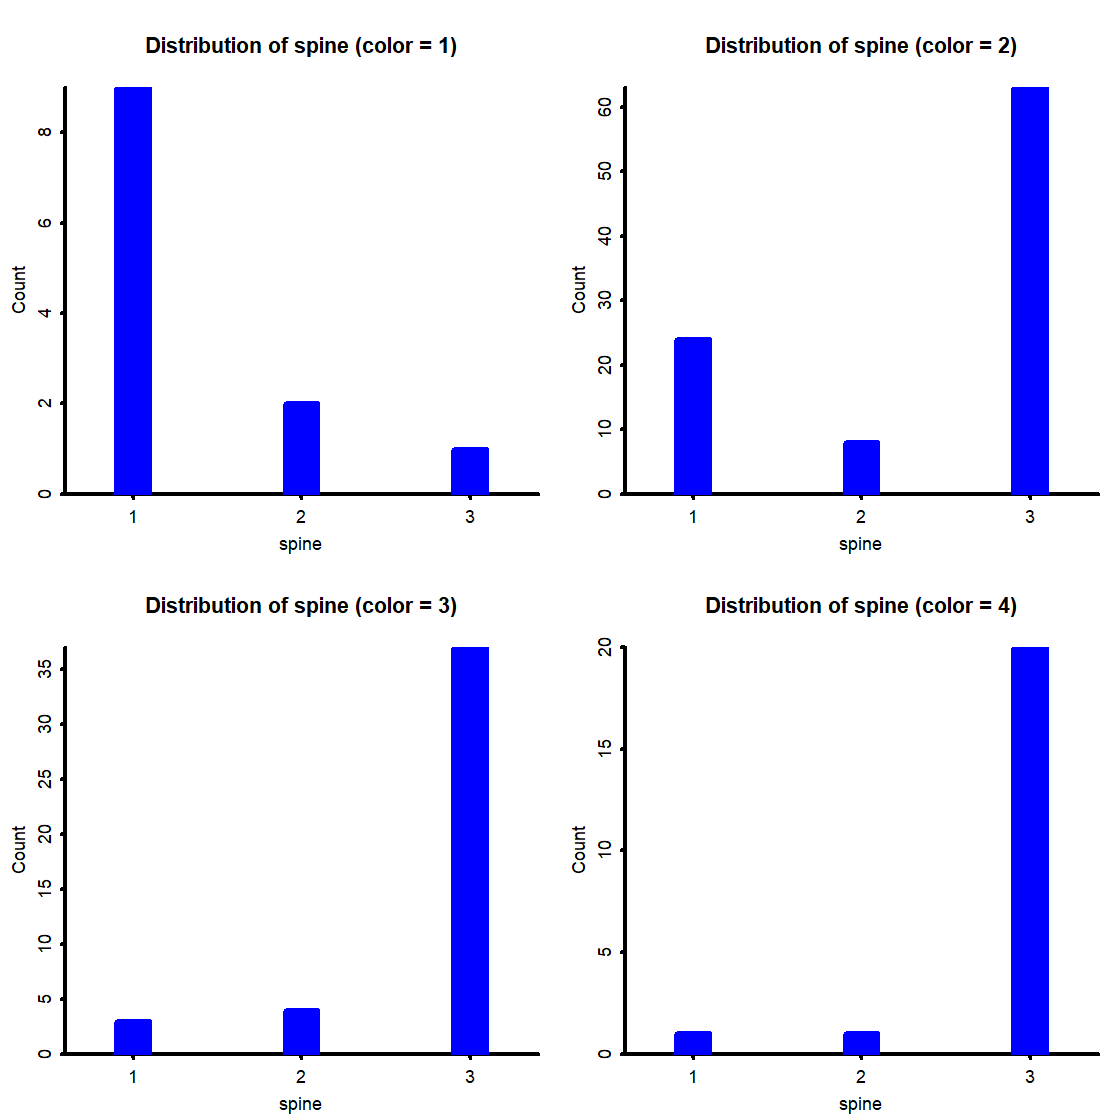
\includegraphics[scale=1.4]{initial-data-analysis/distribution-of-spine-wrt-color}
\caption{Histogram to illustrate the distribution of \texttt{spine} when \texttt{color = 1}, \texttt{color = 2}, \texttt{color = 3} and \texttt{color = 4}.The distribution of \texttt{spine} when \texttt{color = 1} is very different compared to when \texttt{color = 2, 3, 4}. Most of the time, when \texttt{color = 1}, \texttt{spine} takes the value \texttt{1}. When \texttt{color} is \texttt{2}, \texttt{3} or \texttt{4}, \texttt{spine} is very likely going to be \texttt{3}. \texttt{spine = 2} occurs much less frequently compared to the other two cases. It appears that \texttt{color} is likely going an important predictor for modeling \texttt{spine}.
}
\label{distribution-of-spine-wrt-color}
\end{center}
\end{figure}

\begin{figure}[H]
\begin{center}
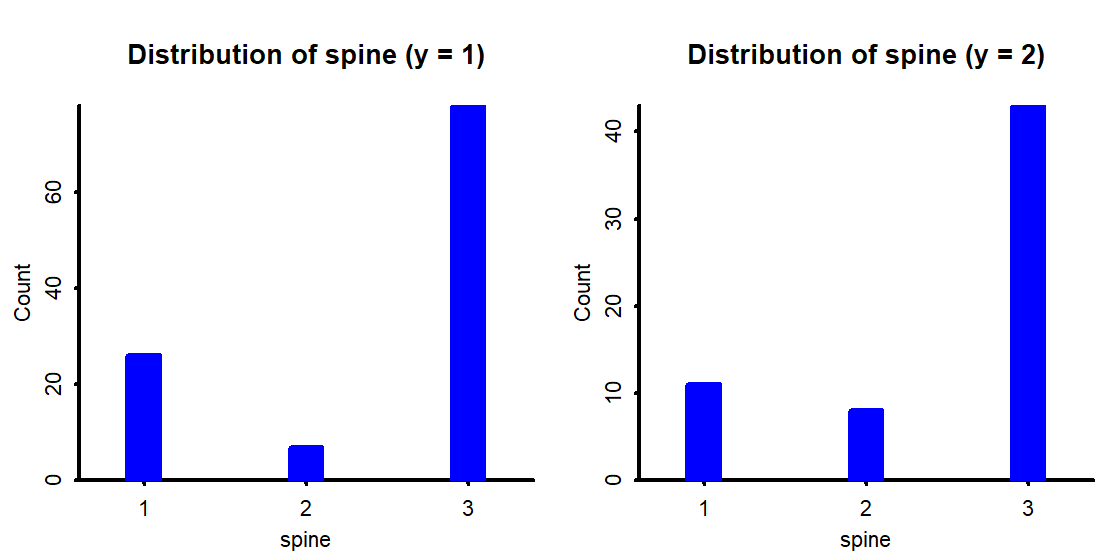
\includegraphics[scale=1.5]{initial-data-analysis/distribution-of-spine-wrt-y}
\caption{Histogram to illustrate the distribution of \texttt{spine} when \texttt{y = 0} and \texttt{y = 1}. These two histograms are very similar in terms of shape. This indicates that the predictor \texttt{y} itself is probably not very useful for predicting \texttt{spine}.
}
\label{distribution-of-spine-wrt-y}
\end{center}
\end{figure}

\subsection{Distribution of \texttt{spine} with respect to 2 variables}
\begin{figure}[H]
\begin{center}
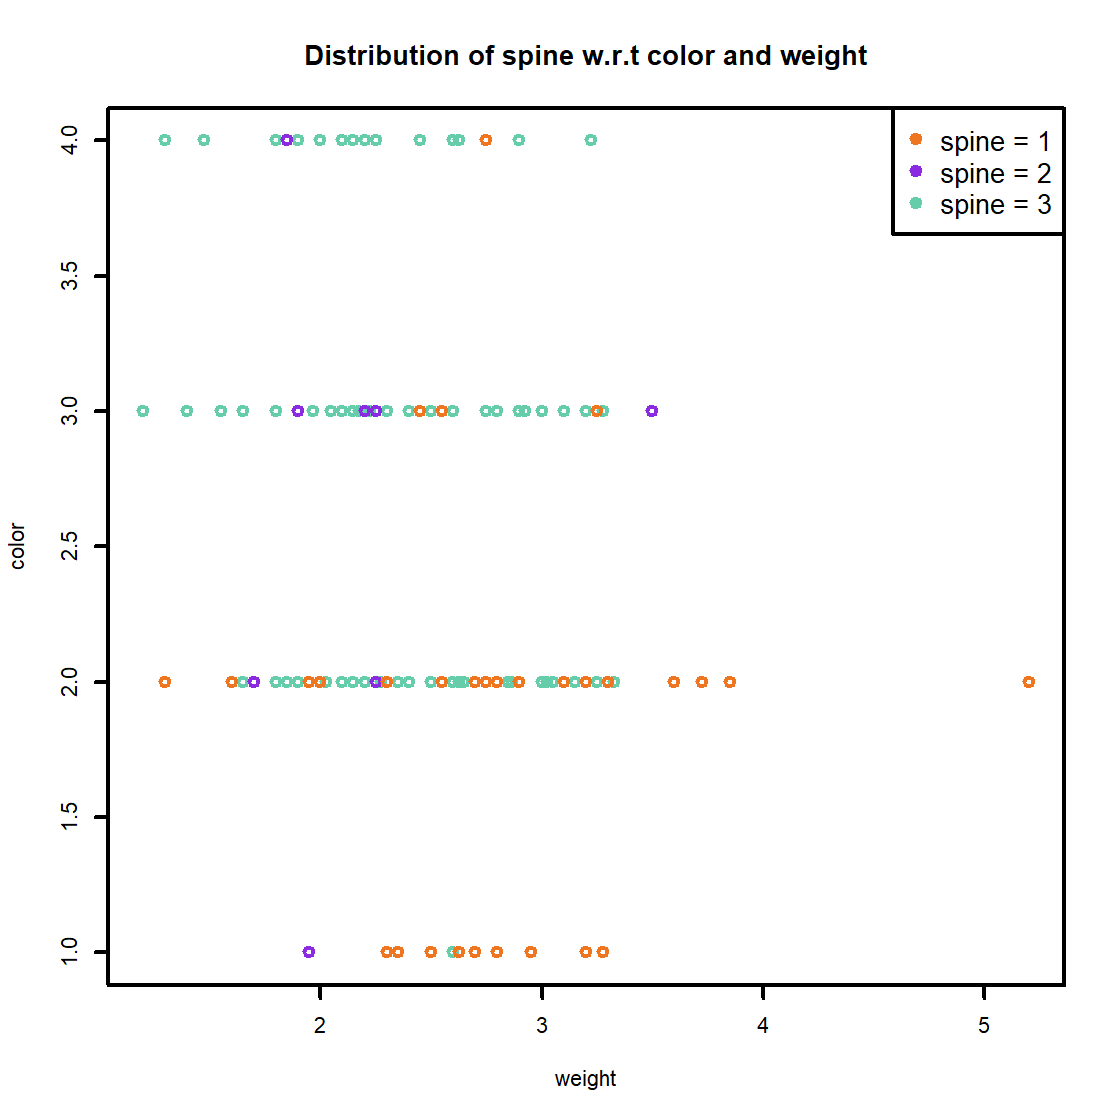
\includegraphics[scale=1.4]{initial-data-analysis/distribution-of-spine-wrt-weight-color}
\caption{Distribution of \texttt{spine} w.r.t \texttt{color} and \texttt{weight}. Orange points (\texttt{spine = 1}) occur more frequently on the bottom-right corner, while green points (\texttt{spine = 3}) are more prevalent on the top half. The fact that we can visually detect a structure might indicate that \texttt{color:weight} is a useful interaction be included in modeling.
}
\label{distribution-of-spine-wrt-2-variables}
\end{center}
\end{figure}

\section{Poisson regression}
\noindent The density function of Poisson distribution can be written as 

\begin{align*}
 P(Y = y) &=
  \begin{cases}
    \frac{\mu^y e^{-\mu} }{y!}        & \text{if } y \in \mathbb{Z^+} \\
   0        & \text{otherwise}
  \end{cases}
  \\
  &=
  \begin{cases}
   \exp(y \log(\mu) - \mu - \log(y!) )& \text{if } y \in \mathbb{Z^+} \\
   0        & \text{otherwise}
  \end{cases}
\end{align*}

\noindent which fulfills equation (1). In a Poisson regression model, $\mu$ is simply $E(Y|X)$, the mean of response variable $Y$ given $X$, and it is associated with the linear predictor $\beta^TX$ via the log link function

$$\log(E(Y|X) = \beta^TX$$

\noindent Since $E(Y|X) = \exp(\beta^TX)$, regardless of the values of $X$, $E(Y|X)$ will always be positive. Additionally, since the distribution of $Y$ given $X$ is Poisson, it follows that 

$$ Var(Y|X) = E(Y|X) = \exp(\beta^TX)$$

\noindent The single parameter $\mu$ in a Poisson distribution defines its entire distribution. This means that, in a Poisson regression model, the linear predictor $\beta^TX$ determines both variance and mean of $Y$. Although this is an elegant formulation, for many datasets, $Var(Y|X)$ may be much larger or smaller than $E(Y|X)$. Fitting a Poisson regression model to such data may lead to \textit{overdispersion} or \textit{underdispersion}. \\
\indent In this section, the goal is to obtain the best possible Poisson regression model to serve as a benchmark before moving on to more complex models.

\subsection{Experimentation}
\subsubsection{Baseline model with all main effects}
The first Poisson model that was attempted includes all main effects available, \texttt{spine = sat + y + weight + width + color}. The summary of coefficients (Figure \ref{poisson_all-variables}) show that estimates of the coefficients of all predictors are not significant at the 0.05 level, except for \texttt{color}. 

\begin{figure}[H]
\begin{center}
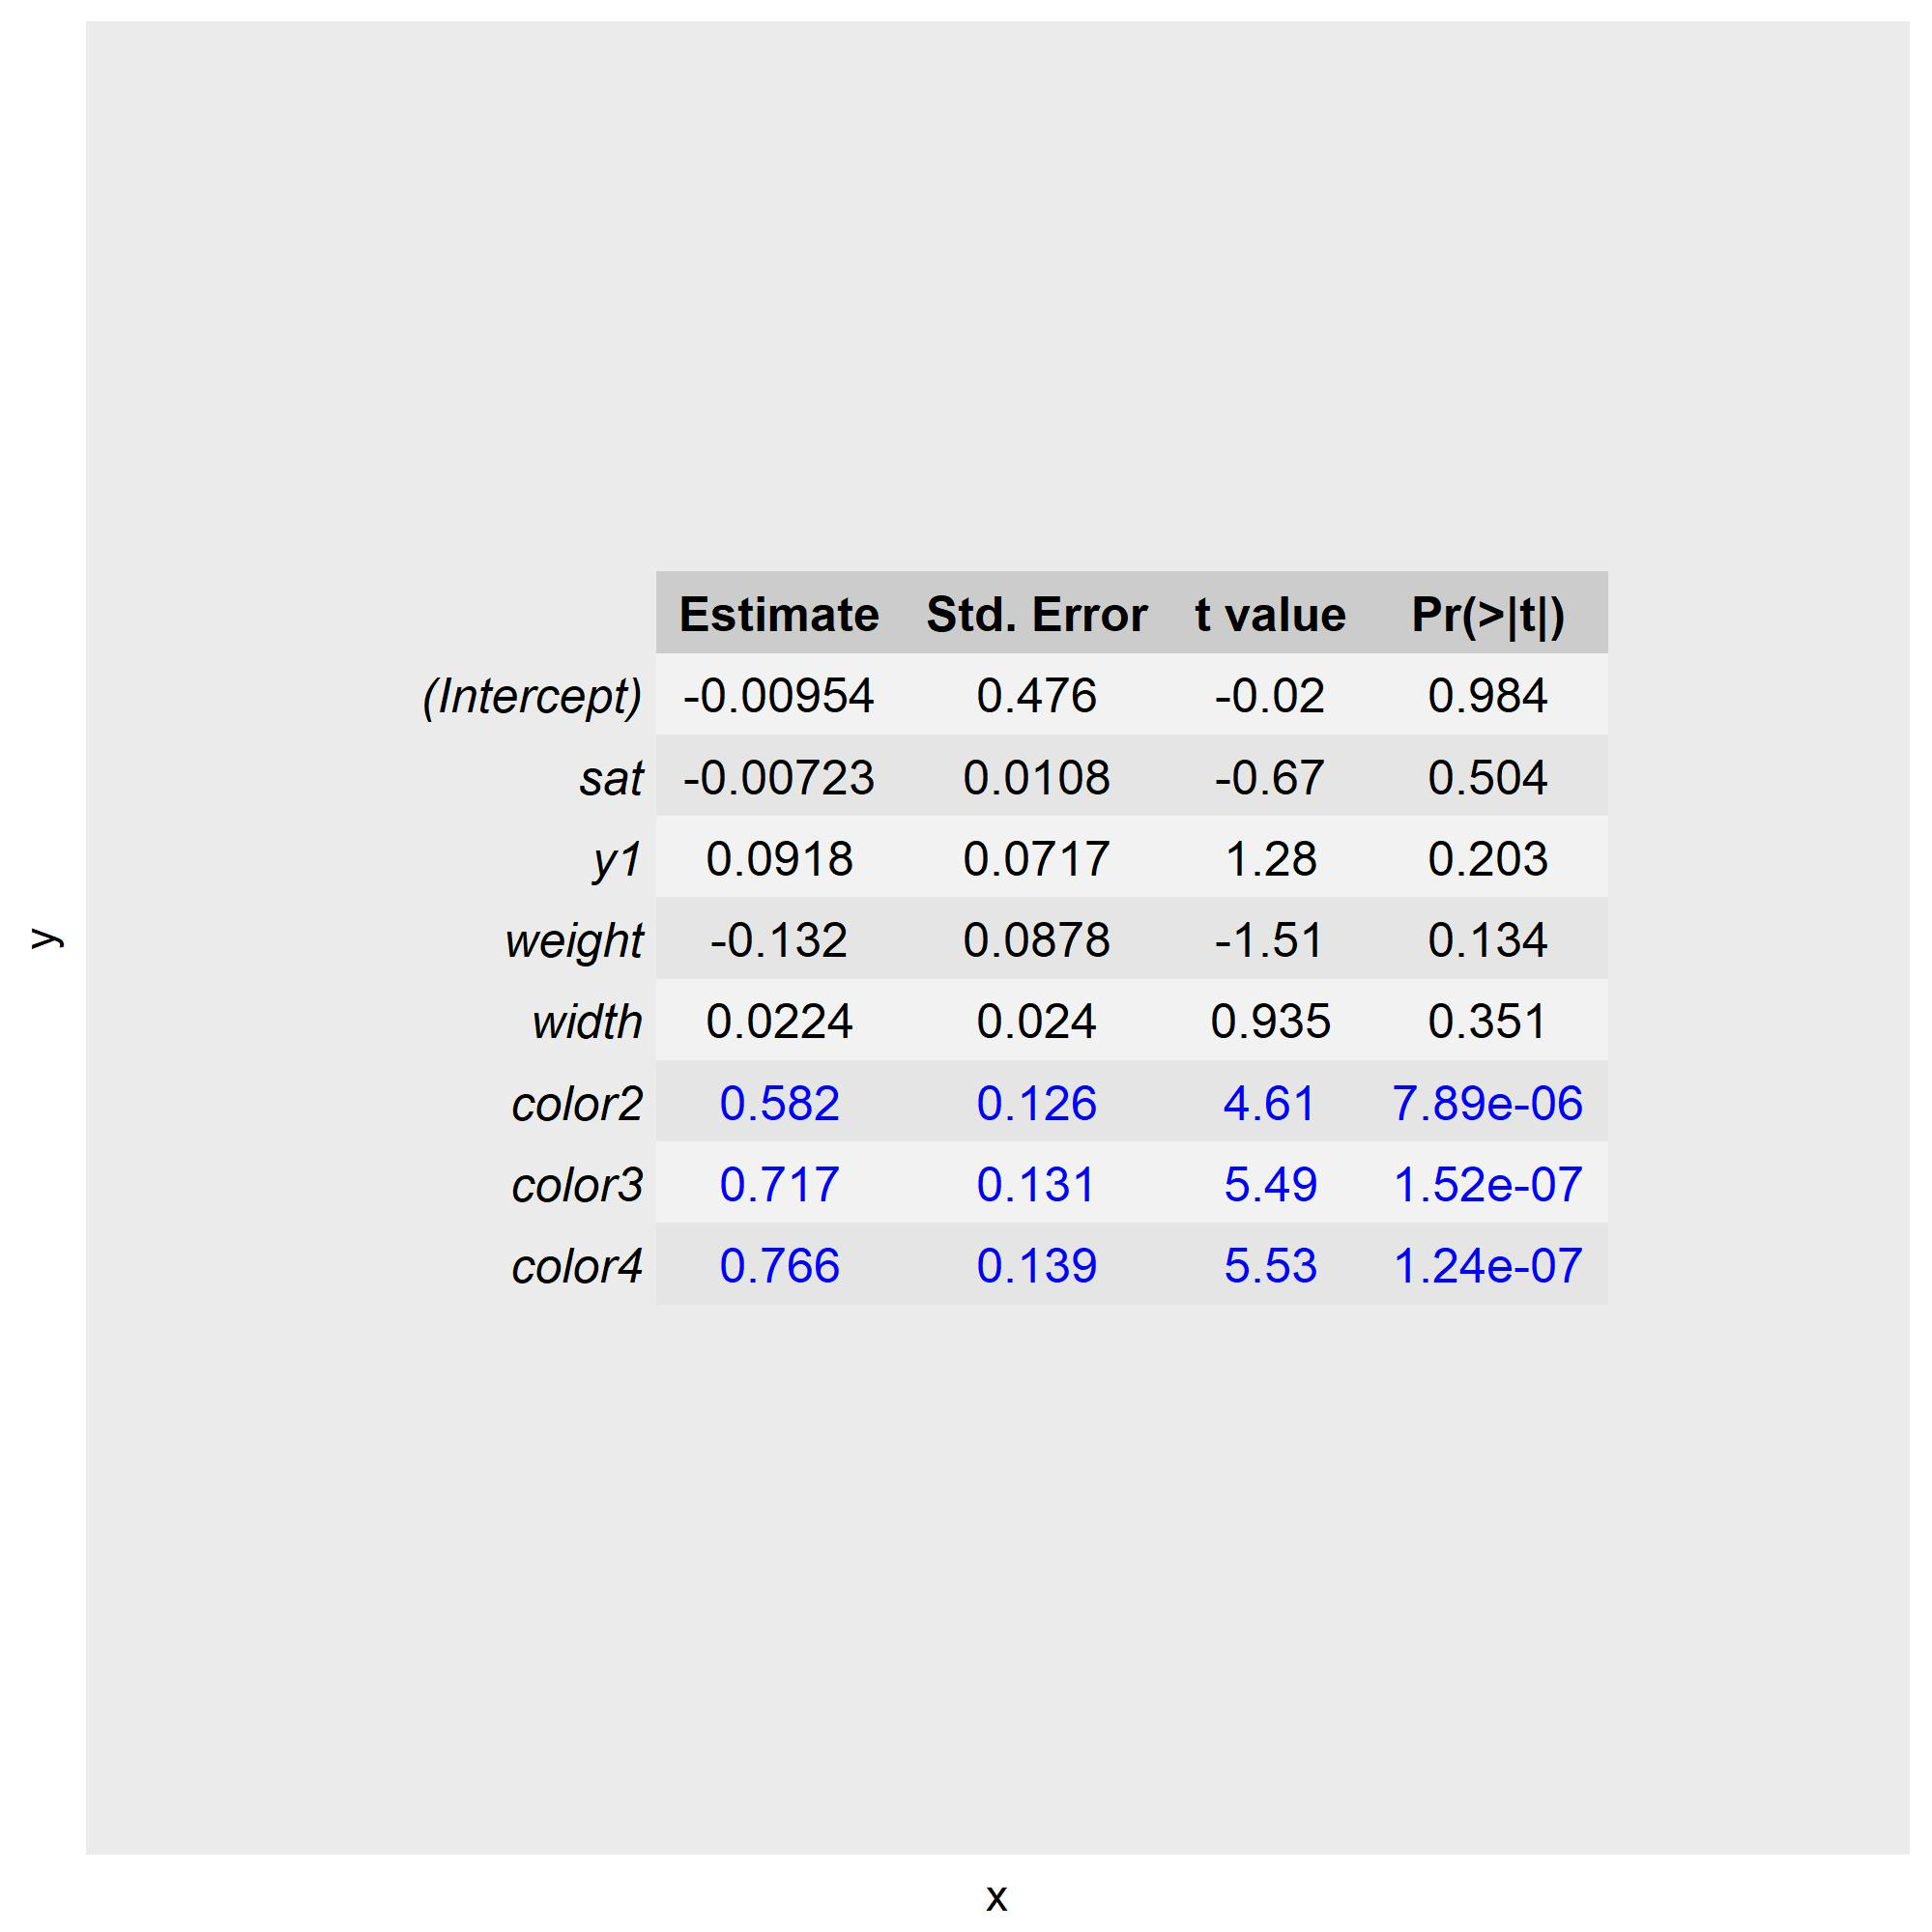
\includegraphics[scale=0.2]{poisson/poisson_all-variables}
\caption{Coefficients of Poisson regression model \texttt{spine = sat + y + weight + width + color}  fitted to dataset. Only indicator variables of \texttt{color} are significant at the 0.05 level.  
}
\label{poisson_all-variables}
\end{center}
\end{figure}

\subsubsection{Single predictor model}
The model \texttt{spine = sat + y + weight + width + color} may be a reference that can be used for comparison later on. Since it is much more difficult to understand a model with large number of predictors, the strategy adopted here is to start with the simplest possible model, and then build upon it. To find such a model, all possible models with single predictor was fitted to the data.     

\begin{figure}[H]
    \centering
    \subfloat[\texttt{spine = weight}]{{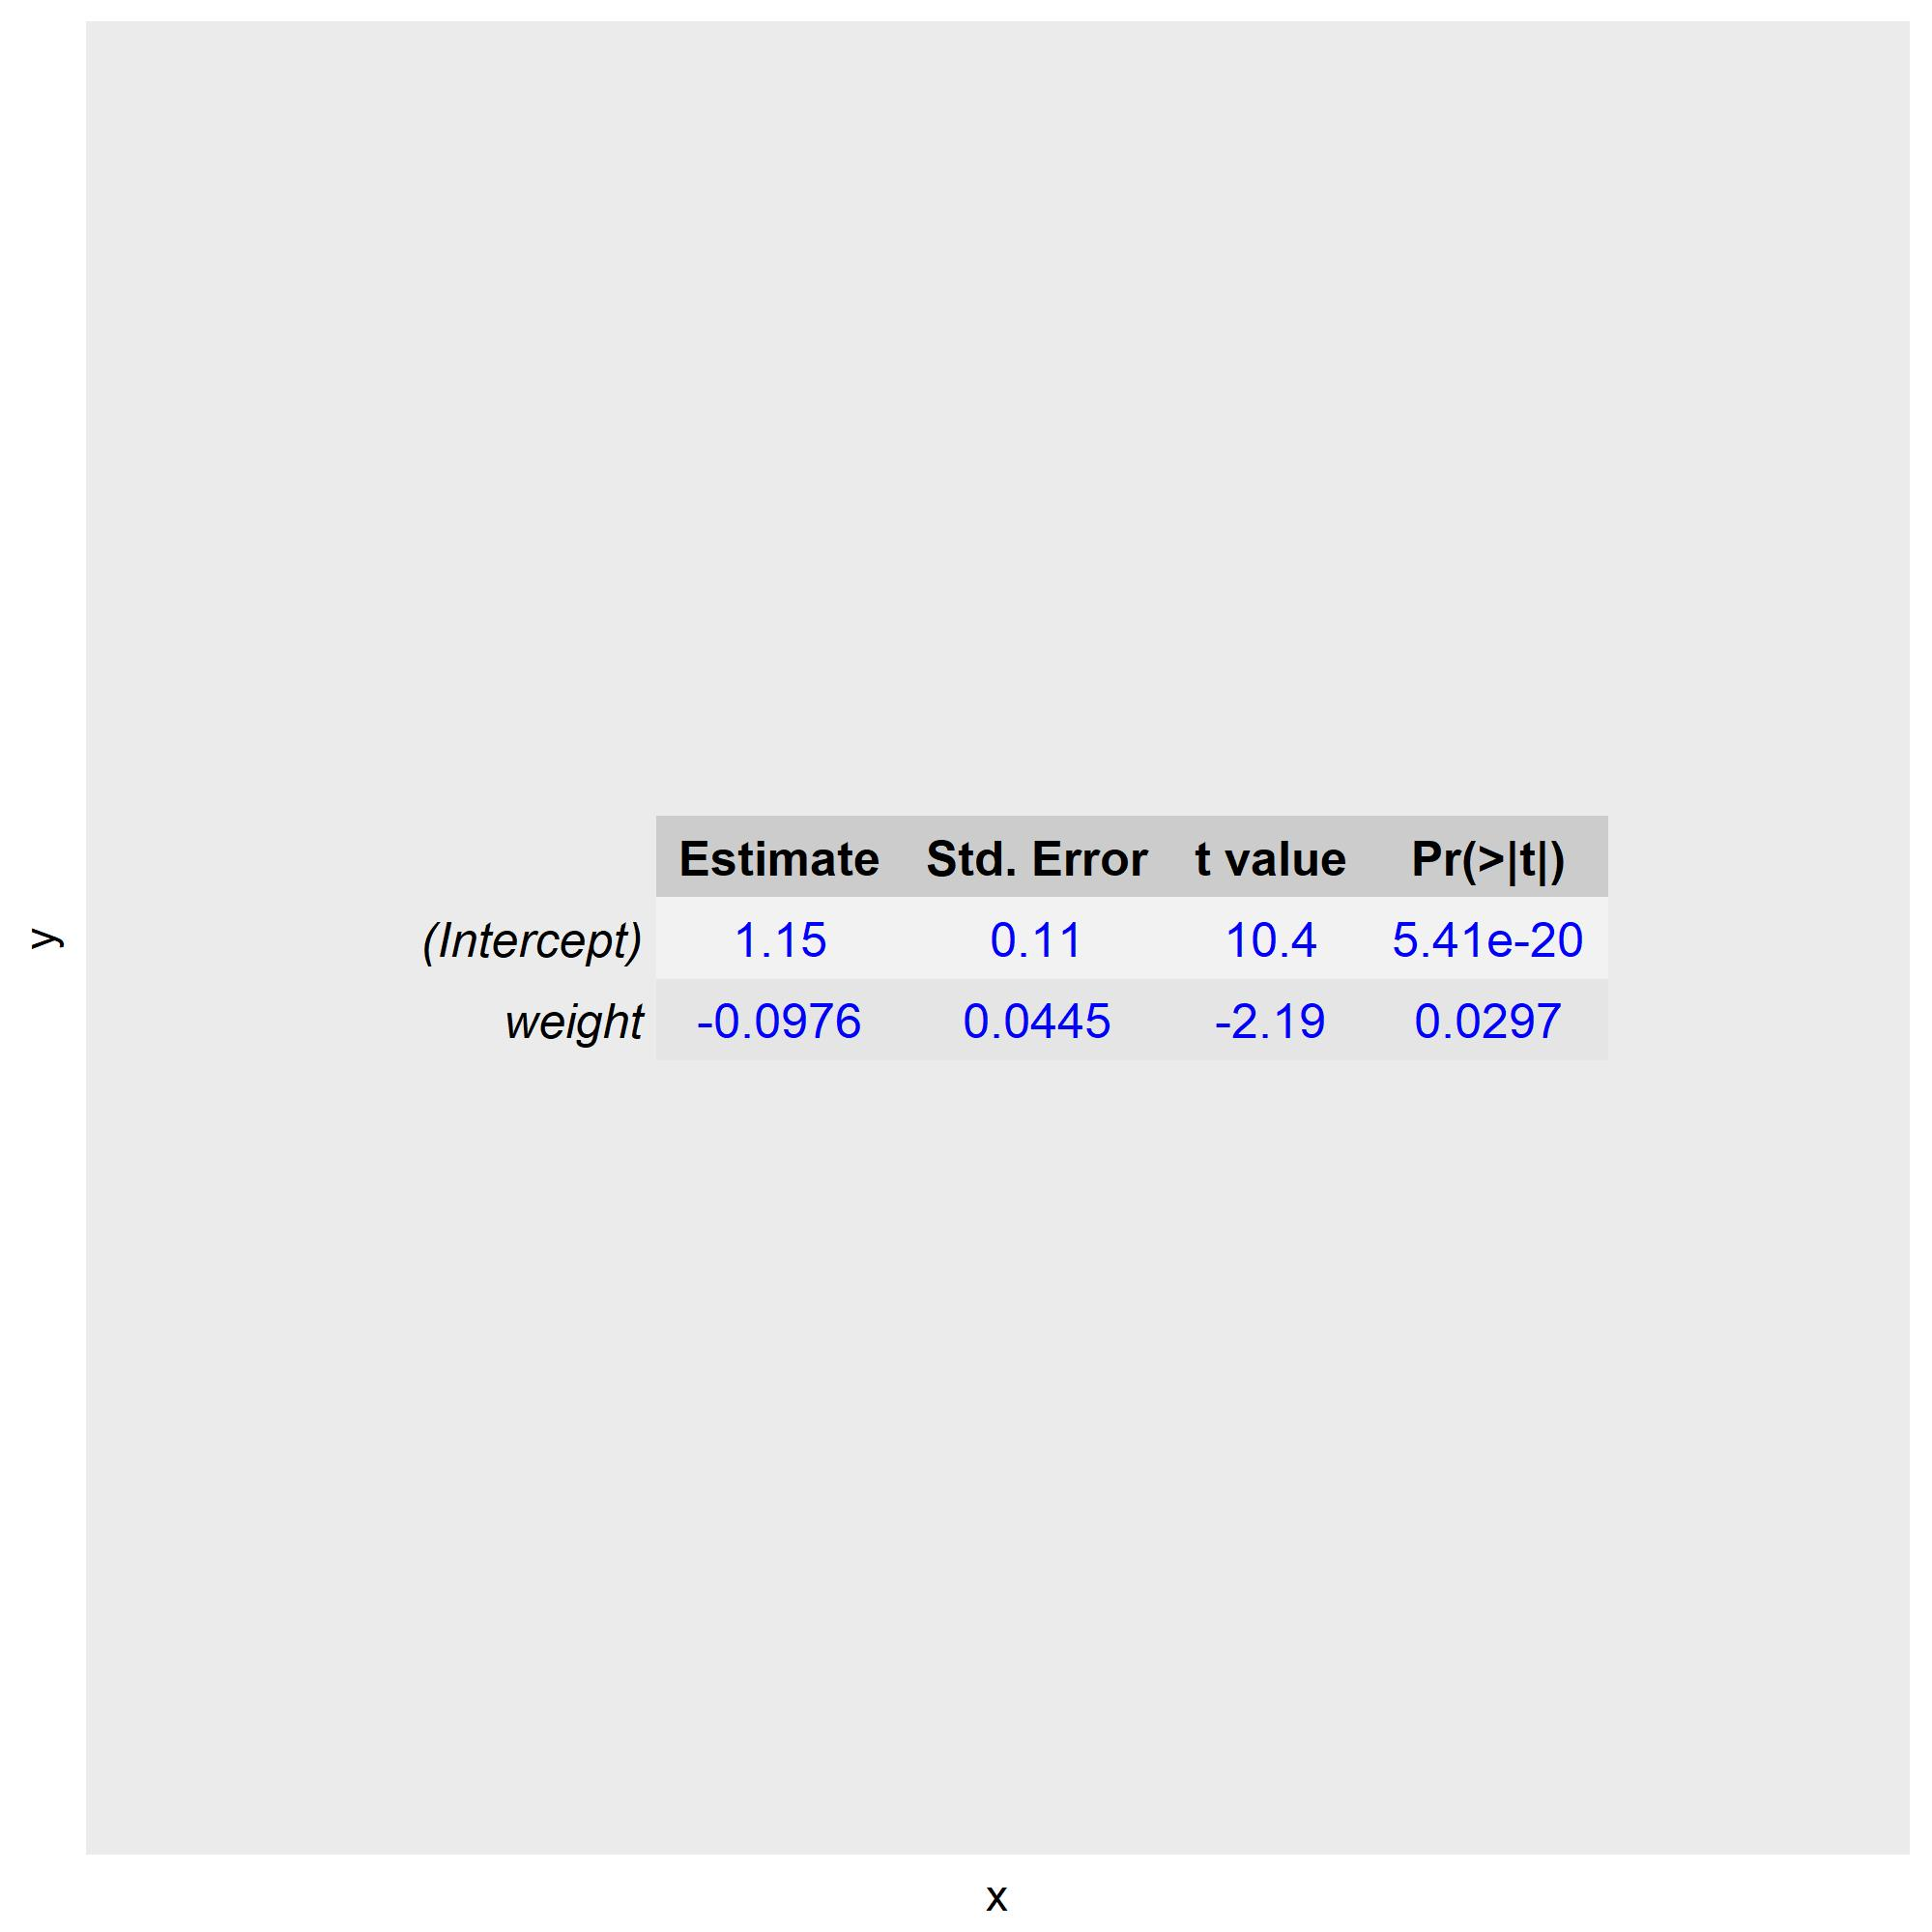
\includegraphics[scale=0.2]{poisson/poisson_weight} }}
    \qquad
    \subfloat[\texttt{spine = y}]{{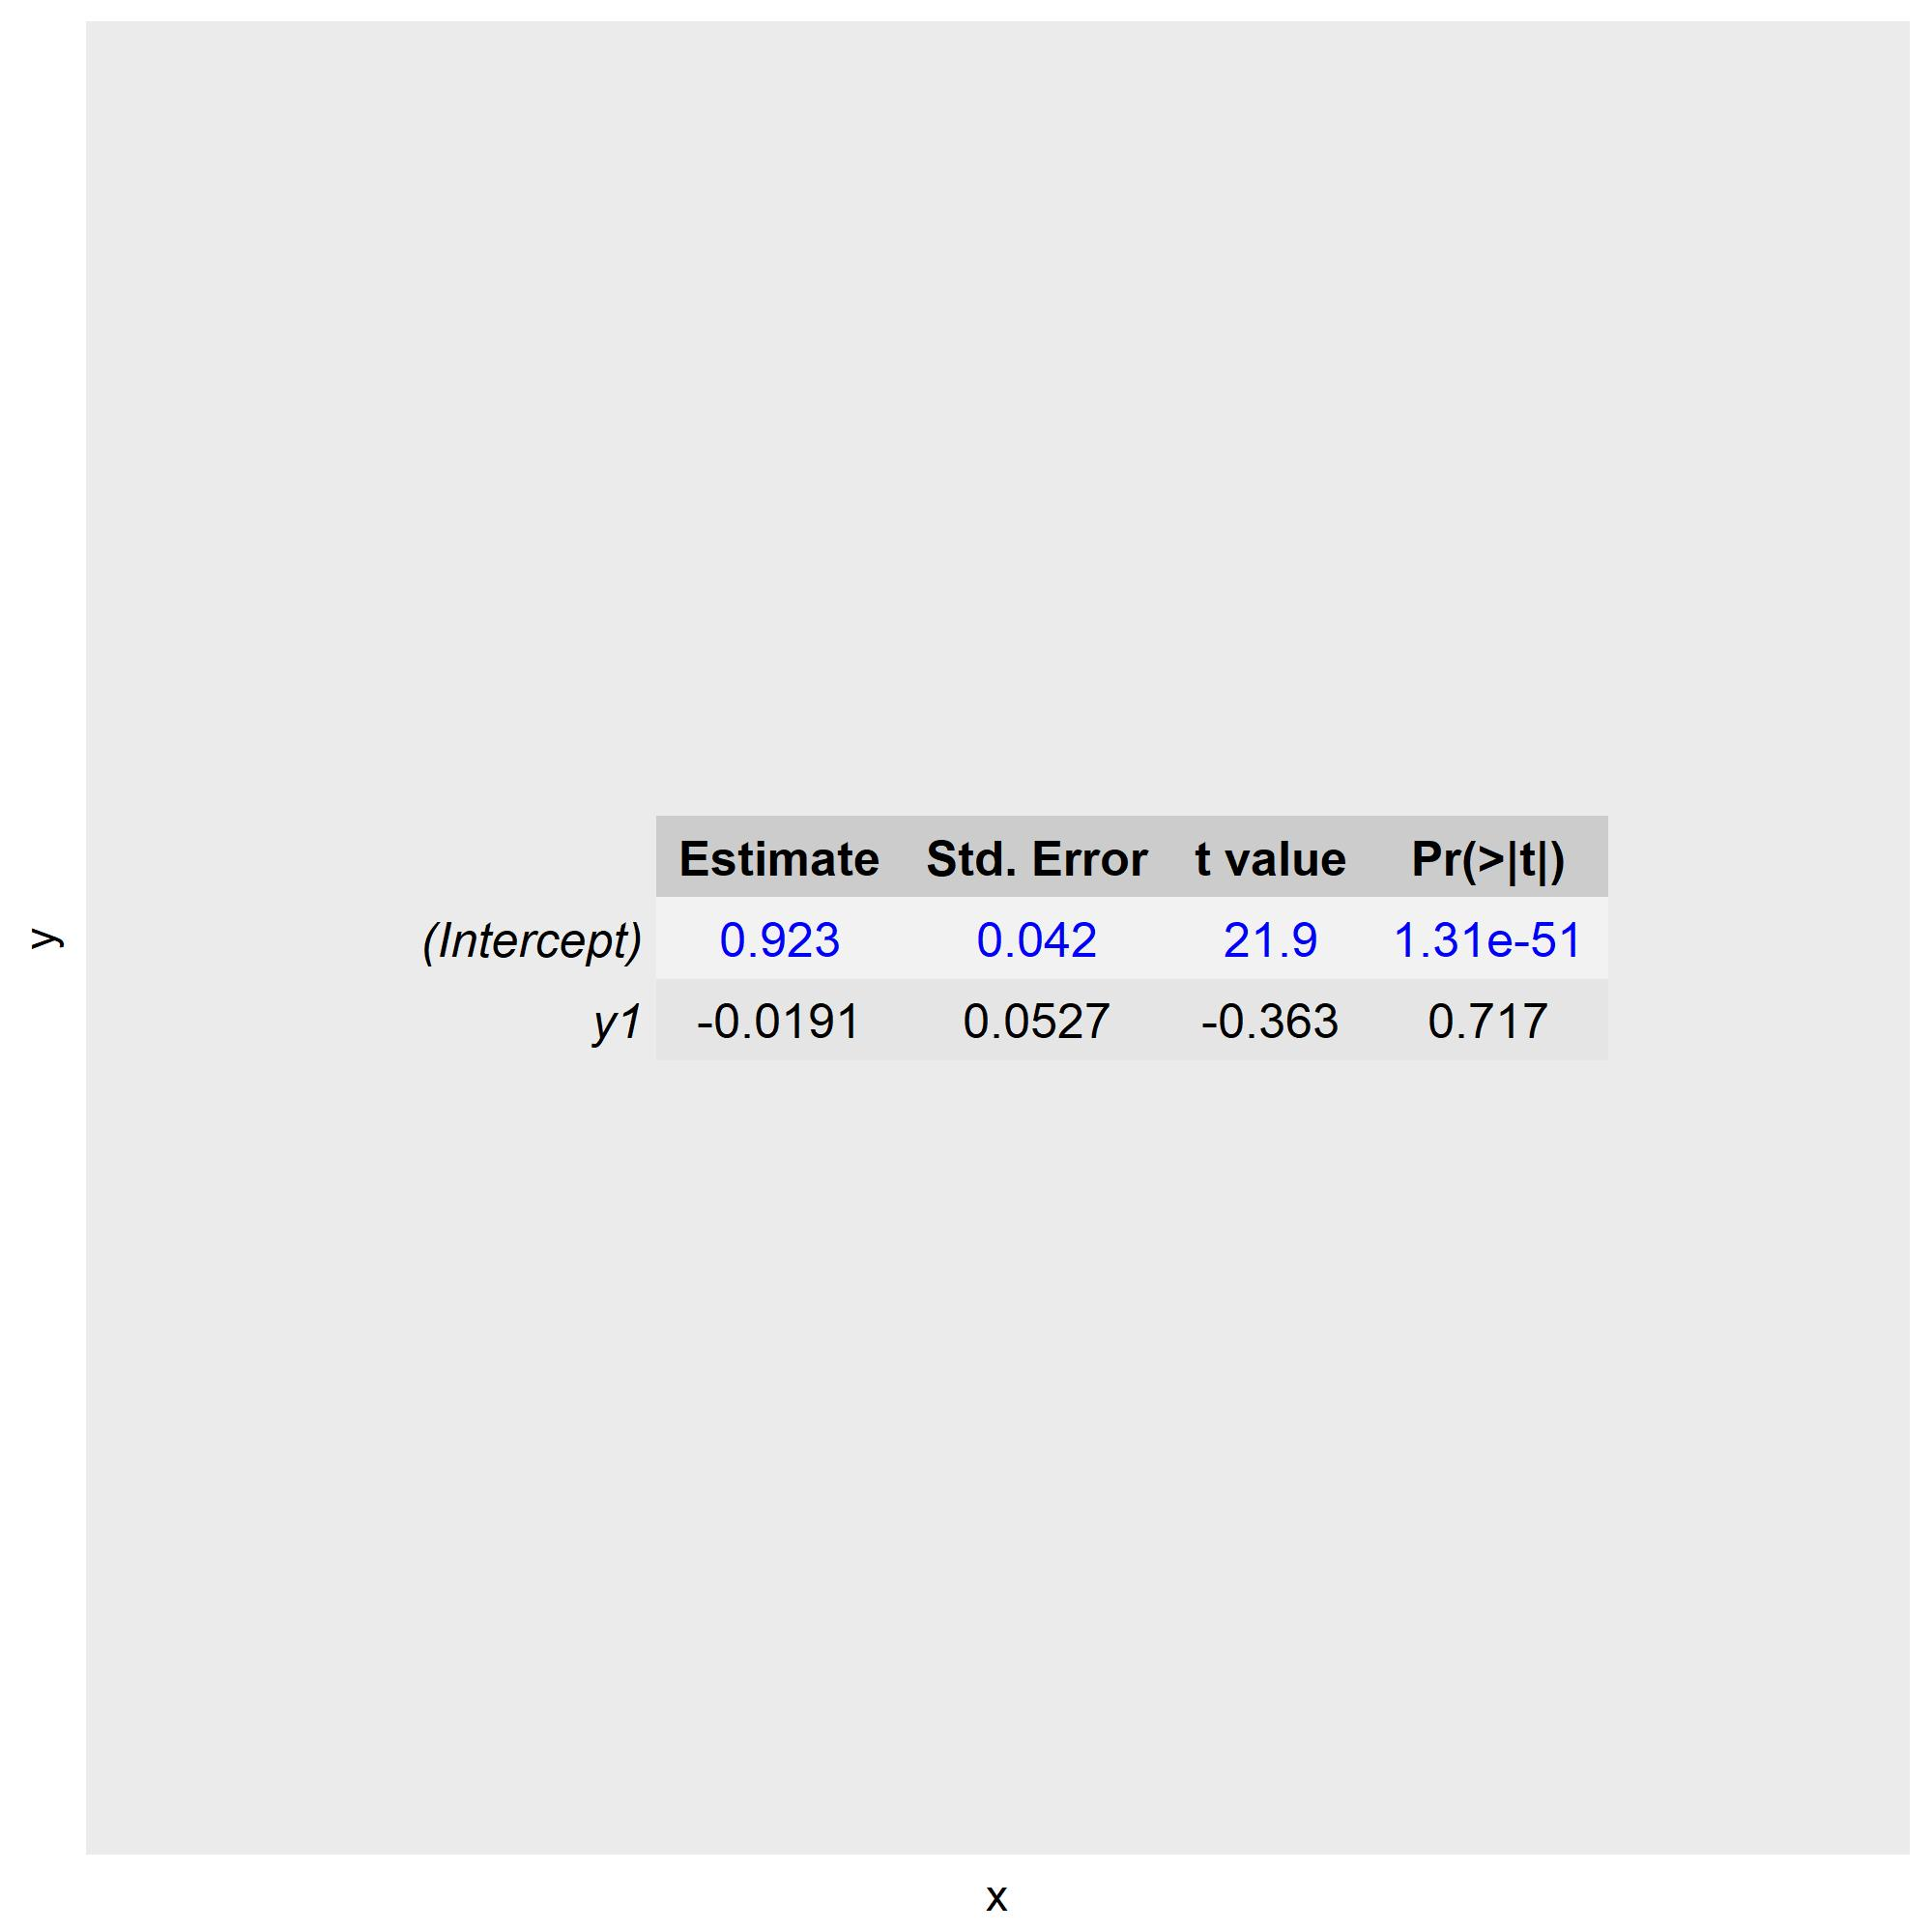
\includegraphics[scale=0.2]{poisson/poisson_y} }}
    \qquad
    \subfloat[\texttt{spine = width}]{{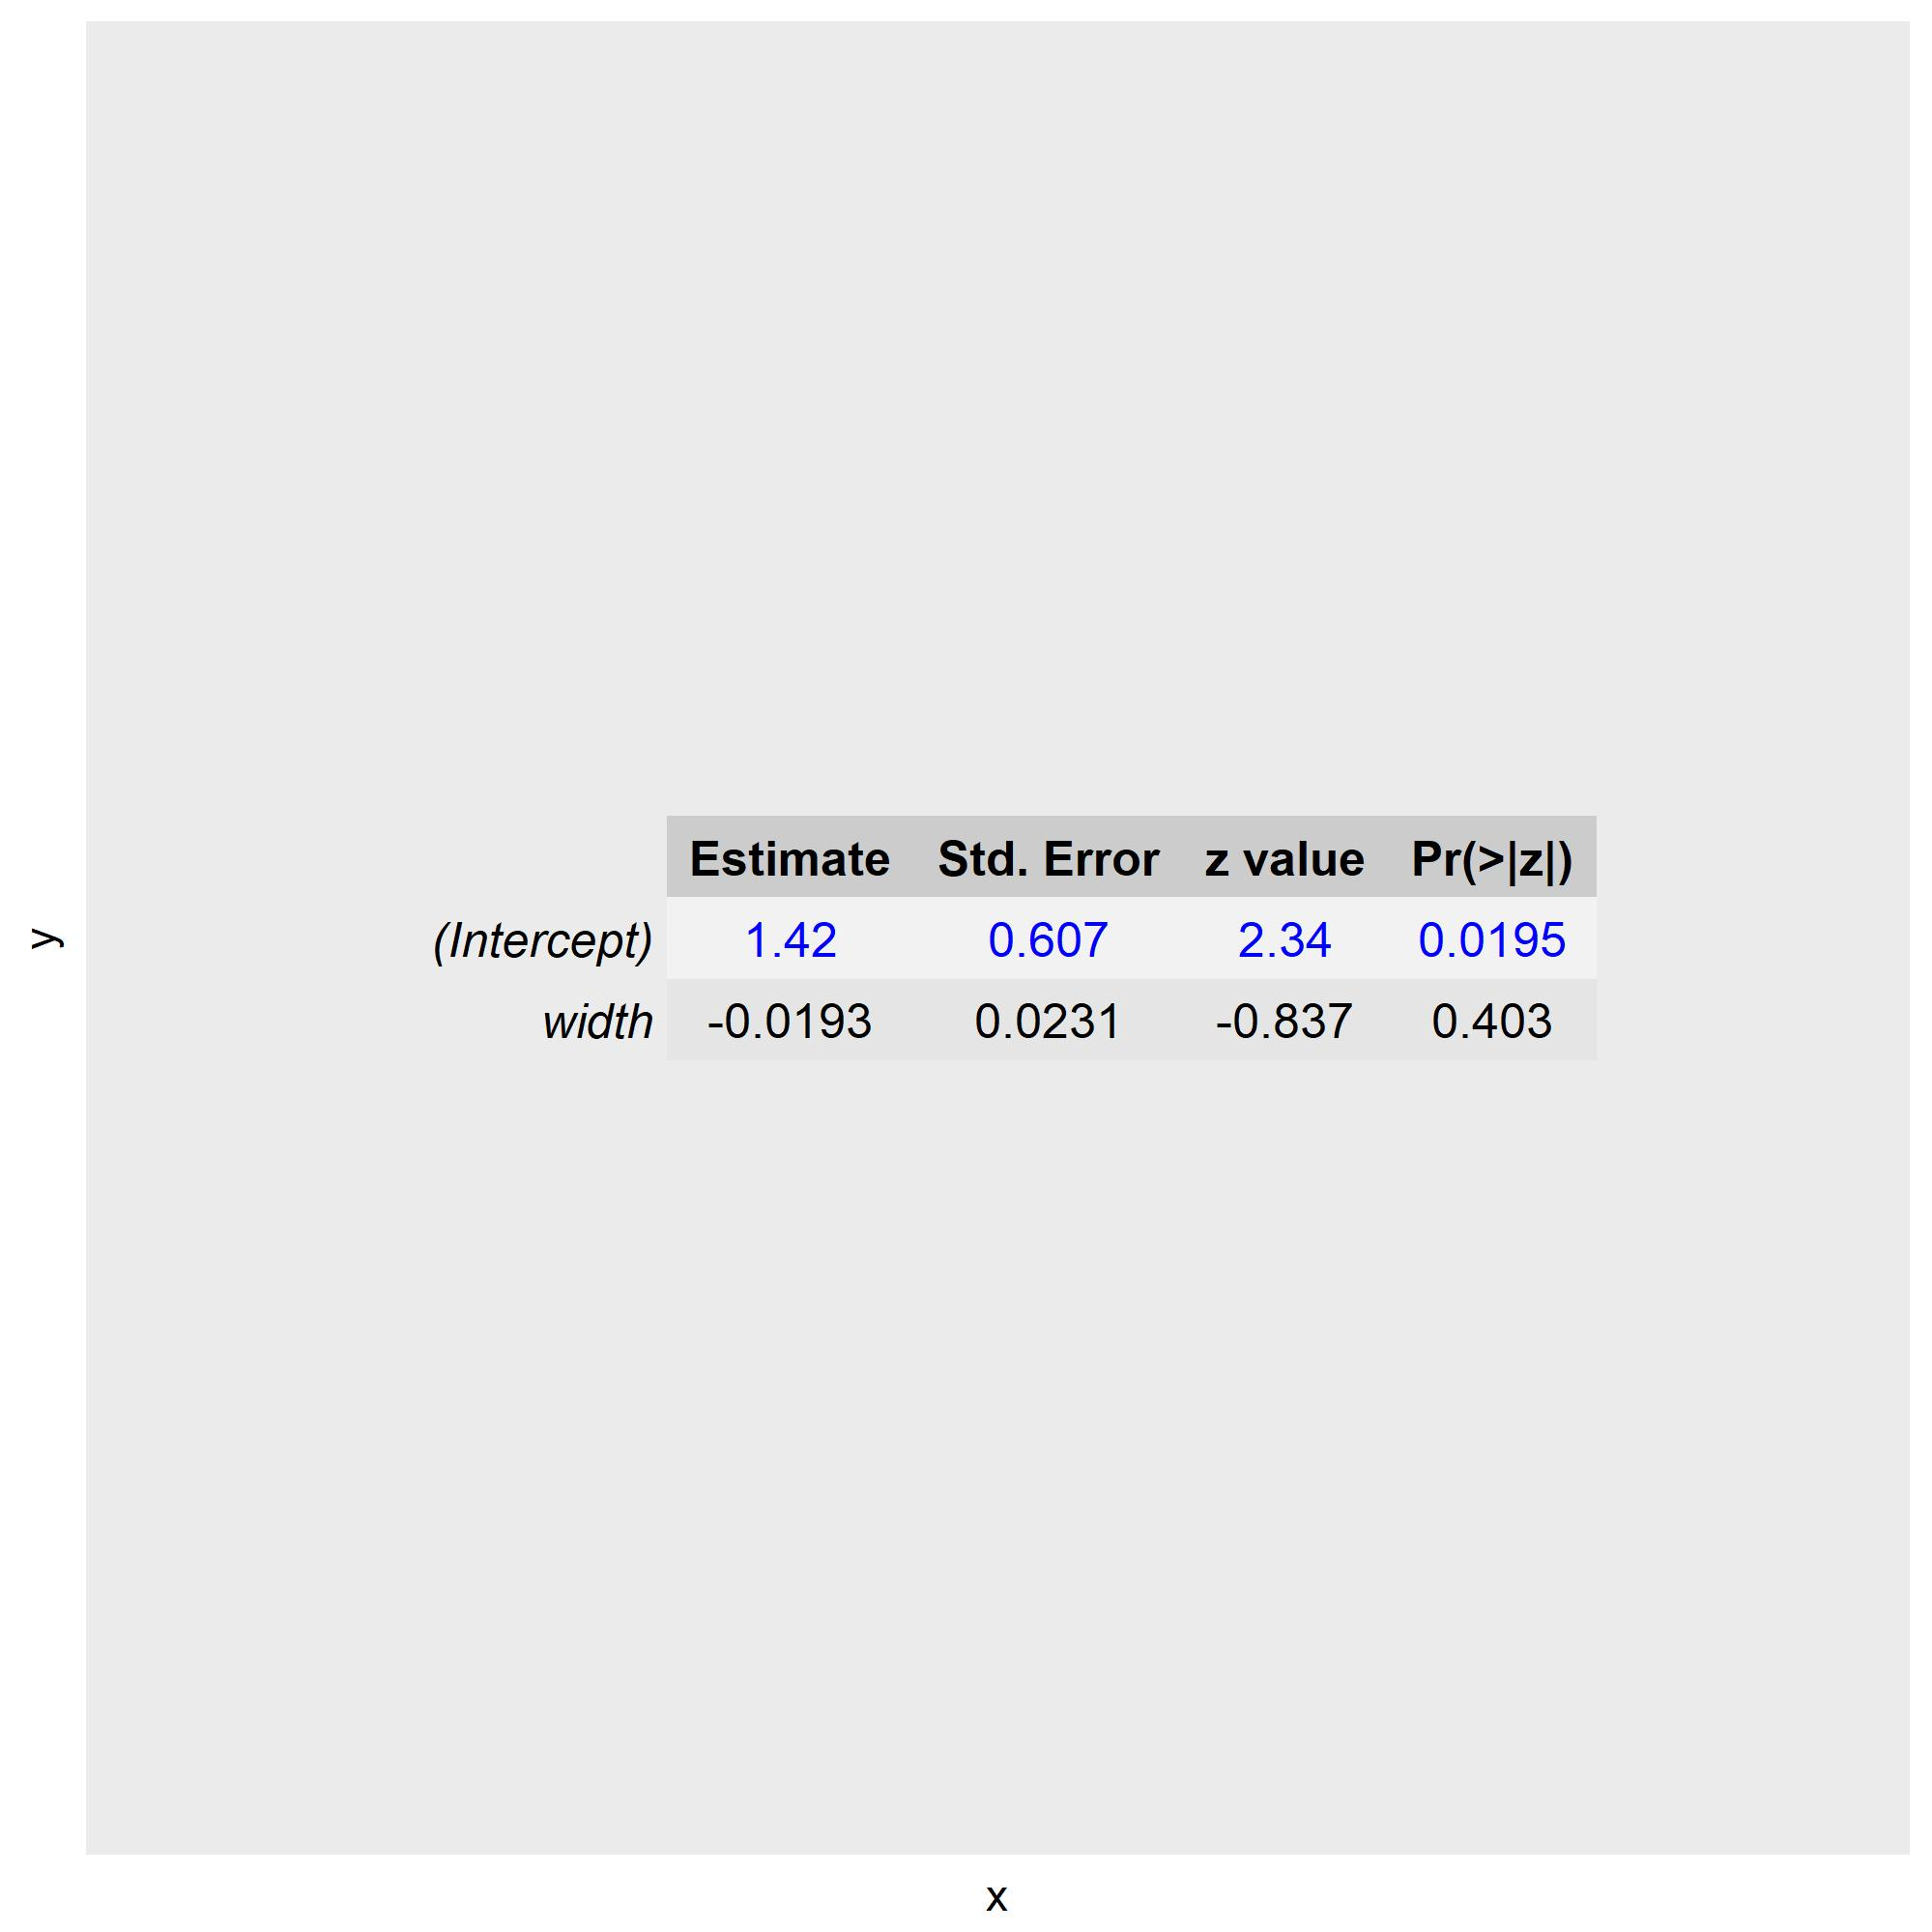
\includegraphics[scale=0.2]{poisson/poisson_width} }}
    \qquad
    \subfloat[\texttt{spine = sat}]{{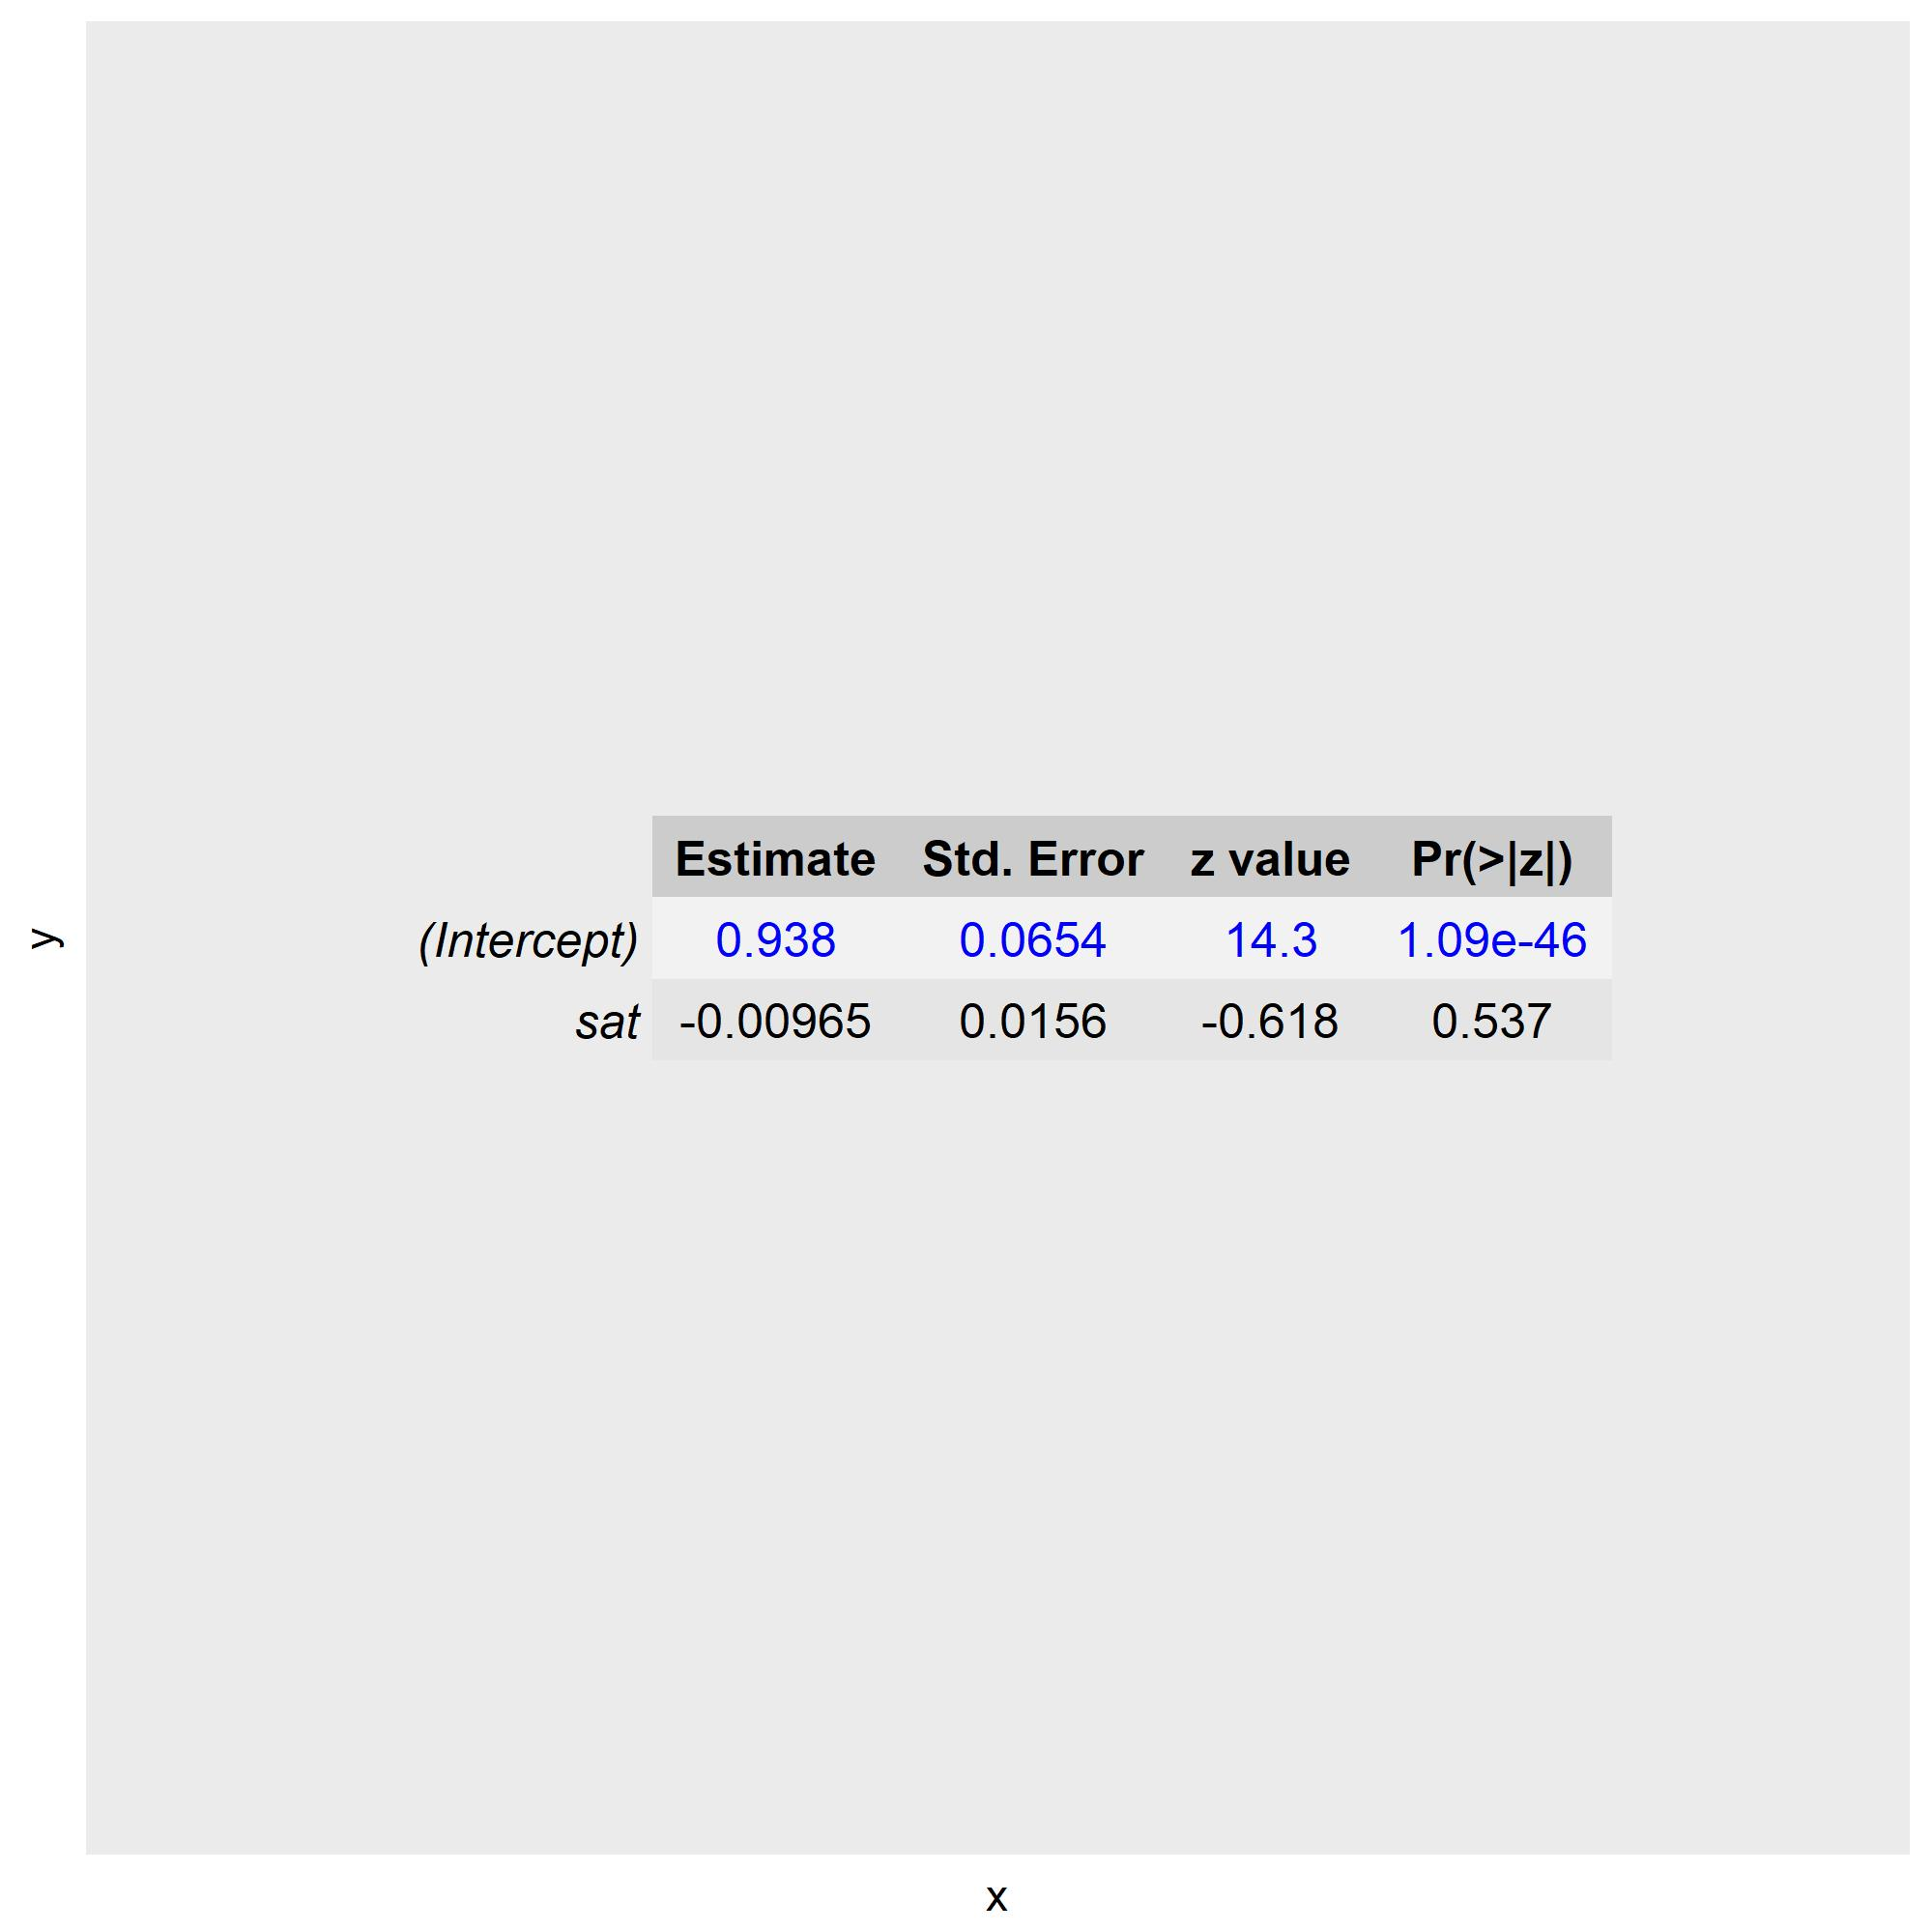
\includegraphics[scale=0.2]{poisson/poisson_sat} }}
    \qquad
    \subfloat[\texttt{spine = color}]{{\includegraphics[scale=0.2]{poisson/poisson_color} }}
    \caption{Coefficients from Poisson regression models with single predictor. \texttt{spine = color} has the best fit here. For models in (a), (b), (c) and (d) the coefficients of predictor variable are all not significant at the 0.05 level.}
    \label{single-predictor-poisson-models}
\end{figure}

Based on Figure \ref{single-predictor-poisson-models}, it is clear that \texttt{color} is the most important variable for predicting \texttt{spine}. To further justify this, the \textit{likelihood ratio test} can be used to compare all of the single predictor models against a reduced (or null) model, \texttt{spine = 1}. The null model simply predicts \texttt{spine} using its sample average. \\

\noindent Formally, a likelihood-ratio test is a hypothesis test with 
$$ H_0: \text{reduced model is true}, \quad H_1: \text{alternative model is true}$$
$$ \Delta G^2 = -2(\log(\mathcal{L}_0(\beta_0; X, y)) - \log(\mathcal{L}_1(\beta_1; X, y)) $$
\noindent where $\Delta G^2$ is the test statistic, $\mathcal{L}_0(\beta_0; X, y)$ and $\mathcal{L}_1(\beta_1; X, y)$ are the likelihoods of null and alternative models. $\Delta G^2$ follows chi-squared distribution with $k$ degrees of freedom, where $k$ is the number of additional coefficients that are present in alternative model but absent in reduced model. Explicit expression of $\Delta G^2$ for likelihood ratio tests between two Poisson models can be derived easily using the expression for likelihood function of a Poisson model :
$$\mathcal{L}(\beta; X, y) = {\displaystyle \prod_{i=1}^{n}  \frac{{\exp(\beta^TX_i})^{y_i} e^{-\exp(\beta^TX_i)} }{y_i!}}$$

\noindent The likelihood-ratio test can only be used if the reduced and alternative models are nested, otherwise $\Delta G^2$ will no longer follow chi-squared distribution. In our case, \texttt{spine = 1} is a valid reduced model for all other Poisson models discussed so far. Additionally, this also allows us to use the AIC, which is defined as 

$$\text{AIC} = 2p - \log(\mathcal{L}(\beta; X, y)), \quad p = \text{number of estimated parameters}$$

\noindent to compare \texttt{spine = 1} with every other Poisson model. Table 2 illustrates the results of likelihood ratio tests and AIC values. 

% Table generated by Excel2LaTeX from sheet 'Poisson'
\begin{table}[htbp]
  \centering
    \begin{tabular}{|c|c|c|c|c|c|c|}
    \toprule
    \multicolumn{2}{|p{12.445em}|}{Model} & \multicolumn{2}{p{8em}|}{Log-likelihood} & \multicolumn{2}{p{8em}|}{AIC} & \multicolumn{1}{c|}{\multirow{2}[4]{*}{LR test: P-value}} \\
\cmidrule{1-6}    \multicolumn{1}{|p{4.5em}|}{Reduced} & \multicolumn{1}{p{7.945em}|}{Proposed} & \multicolumn{1}{p{4em}|}{Reduced} & Proposed & \multicolumn{1}{p{4em}|}{Reduced} & Proposed &  \\
    \midrule
    spine = 1  & \multicolumn{1}{p{7.945em}|}{spine = sat + y + weight + width + color } & -265.69 & -259.91 & 533.38 & 535.82 & 0.12 \\
    spine = 1  & spine = color  & -265.69 & -260.41 & \cellcolor[rgb]{ 1,  .949,  .8}533.38 & \cellcolor[rgb]{ 1,  .949,  .8}528.82 & \cellcolor[rgb]{ 1,  .78,  .808}\textcolor[rgb]{ .612,  0,  .024}{0.01} \\
    spine = 1  & spine = weight  & -265.69 & -265.03 & 533.38 & 534.05 & 0.25 \\
    spine = 1  & spine = width  & -265.69 & -265.34 & 533.38 & 534.67 & 0.40 \\
    spine = 1  & spine = sat  & -265.69 & -265.50 & 533.38 & 534.99 & 0.53 \\
    spine = 1  & spine = y  & -265.69 & -265.67 & 533.38 & 535.34 & 0.85 \\
    \bottomrule
    \end{tabular}%
    \centering
    \caption*{\textbf{Table 2:} Likelihood-ratio tests and AIC values of each all models with single predictors. Key observations: (a) \texttt{spine = color} is the only single predictor model that passes the likelihood ratio test against null model at 0.05 significance level. (b) \texttt{spine = color} is the only model with lower AIC than null model. (c) Despite having 4 more predictors, \texttt{spine = sat + y + weight + width + color} is only slightly better than \texttt{spine = color} in terms of log likelihood, -259.91 - (-260.41) = 0.5}
\end{table}%

\subsubsection{Improving upon \texttt{spine = color}}

Results from Table 2 confirms that \texttt{spine = color} is the best single predictor model. This is in fact consistent with observations made during exploratory analysis (Figure \ref{distribution-of-spine-wrt-color}). The next step is to consider models of the form \texttt{spine = color + ?}, where \texttt{?} can be any one of \texttt{sat}, \texttt{y}, \texttt{width} or \texttt{weight}. Figure \ref{two-predictor-poisson-models} presents the fitted coefficients for these models.

\begin{figure}[H]
    \centering
    \subfloat[\texttt{spine = color + sat}]{{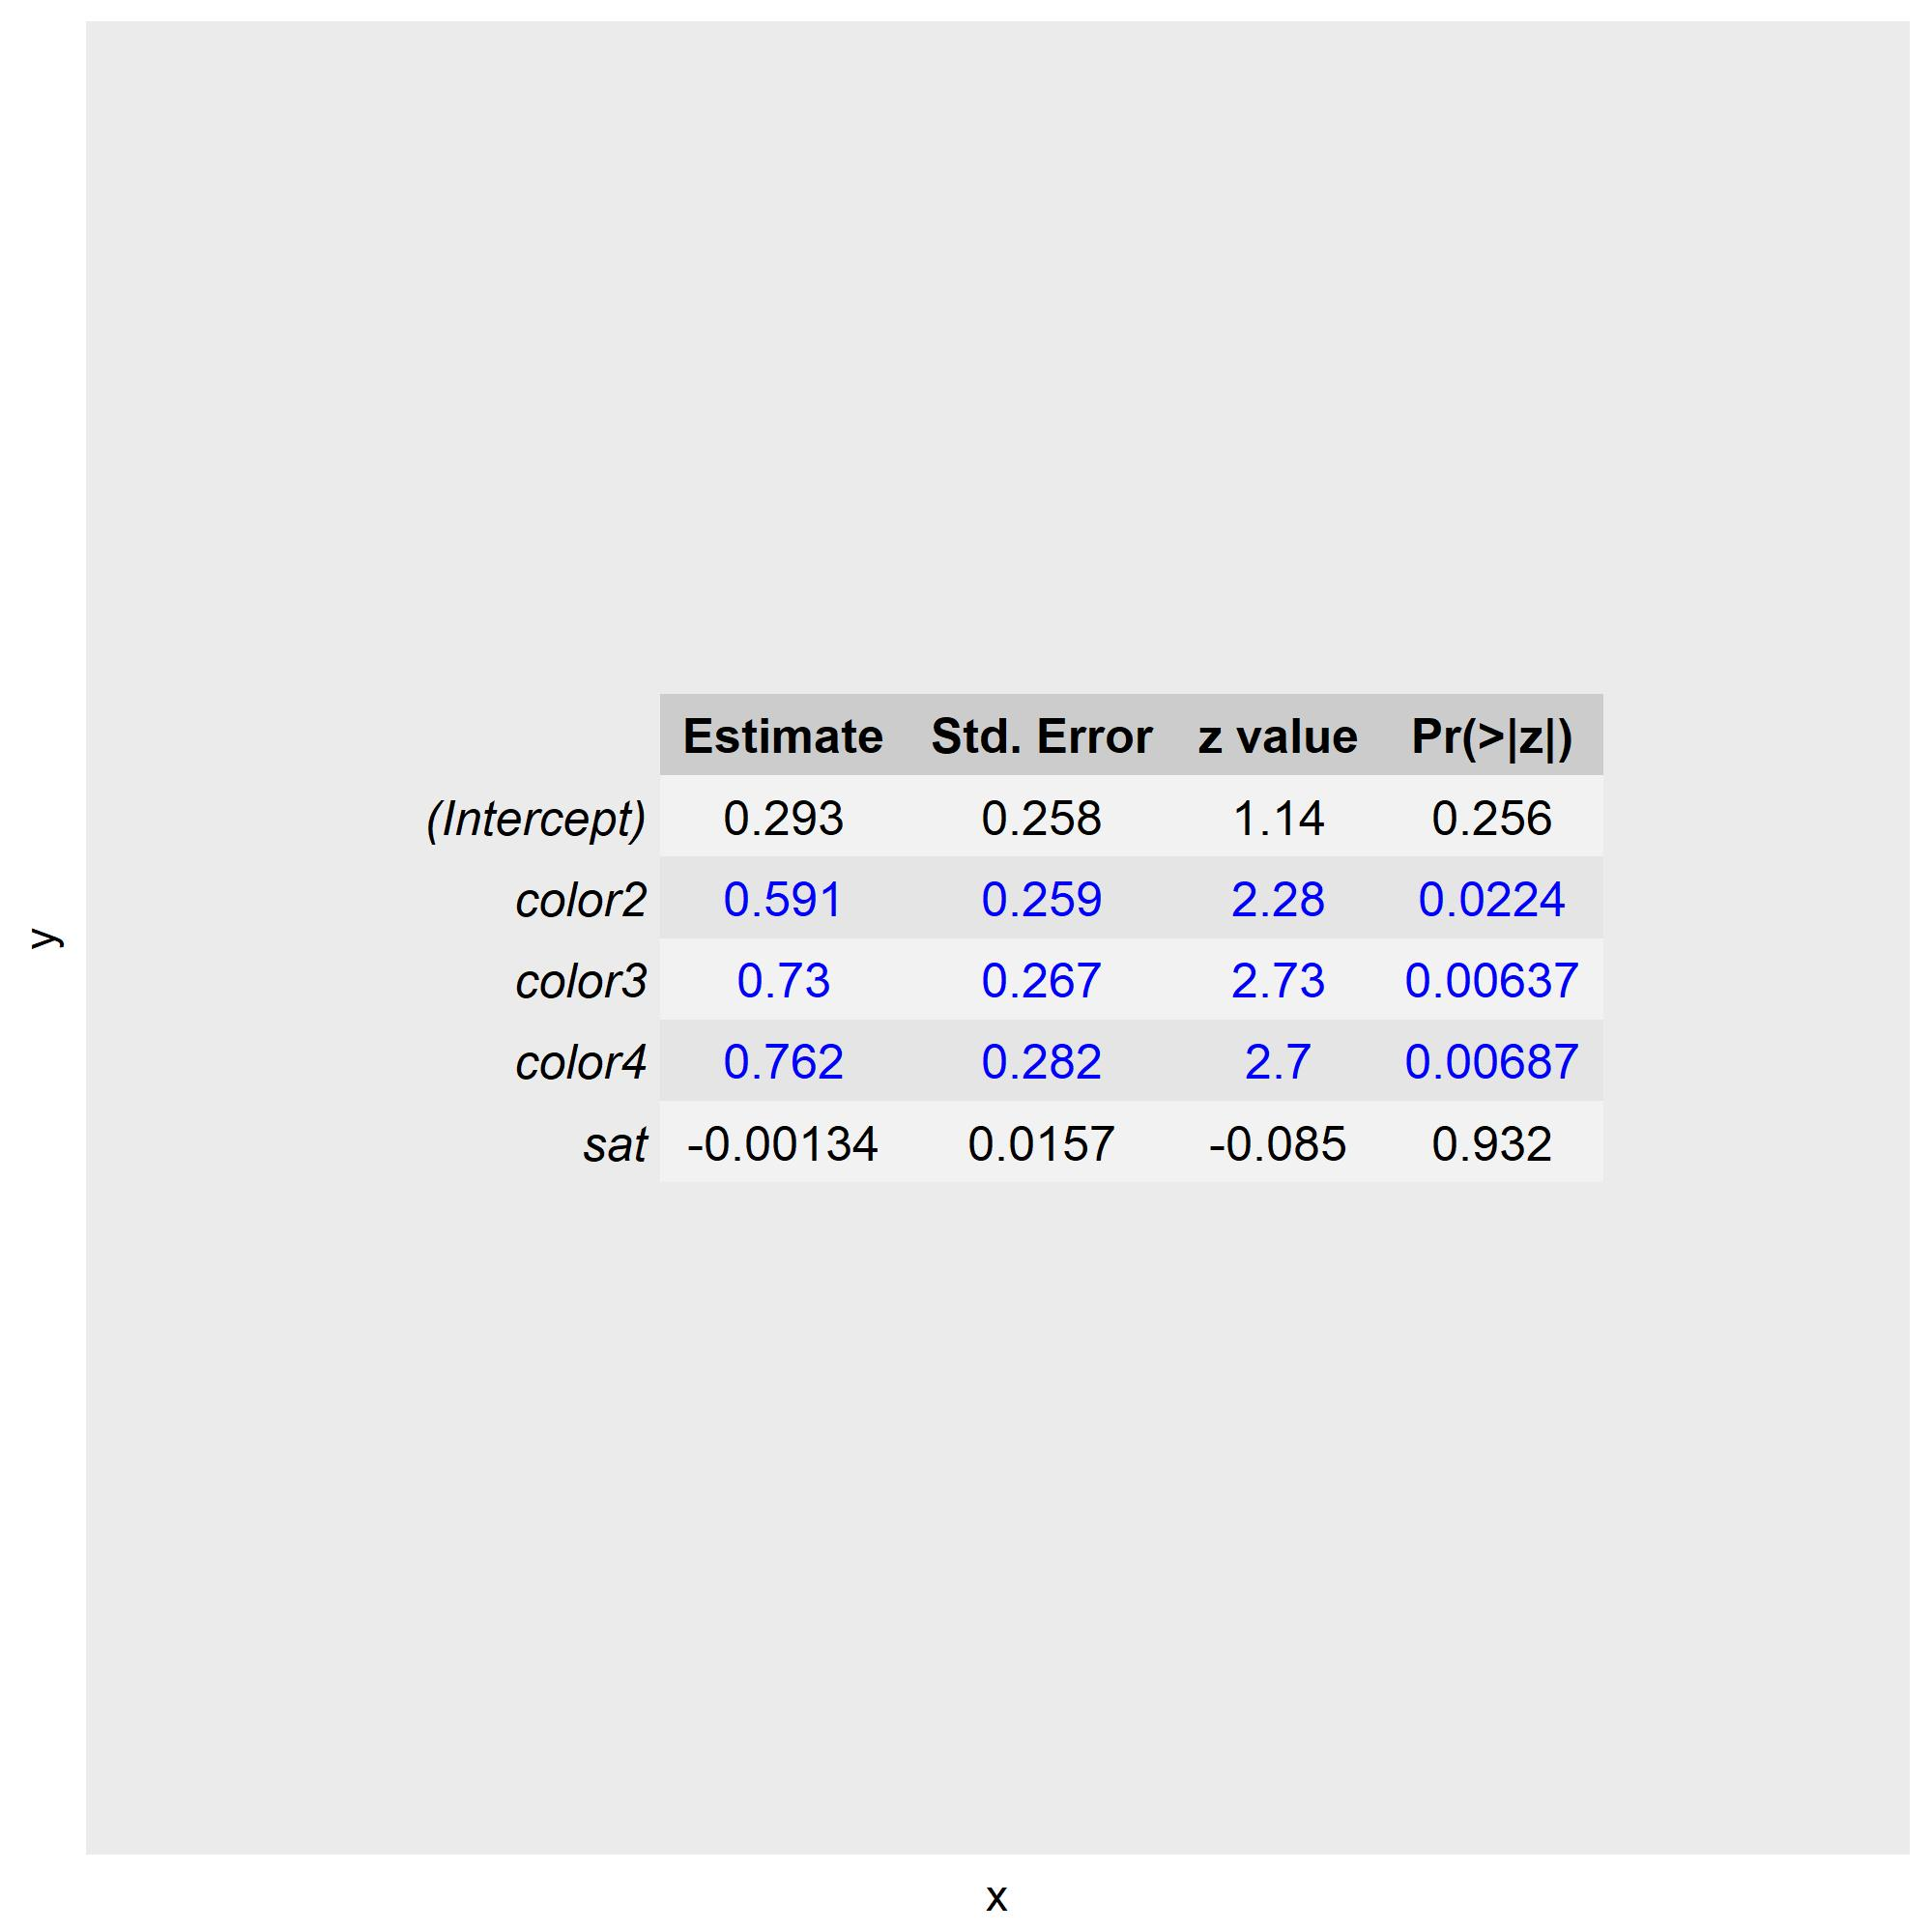
\includegraphics[scale=0.2]{poisson/poisson_color_sat} }}
    \qquad
    \subfloat[\texttt{spine = color + weight}]{{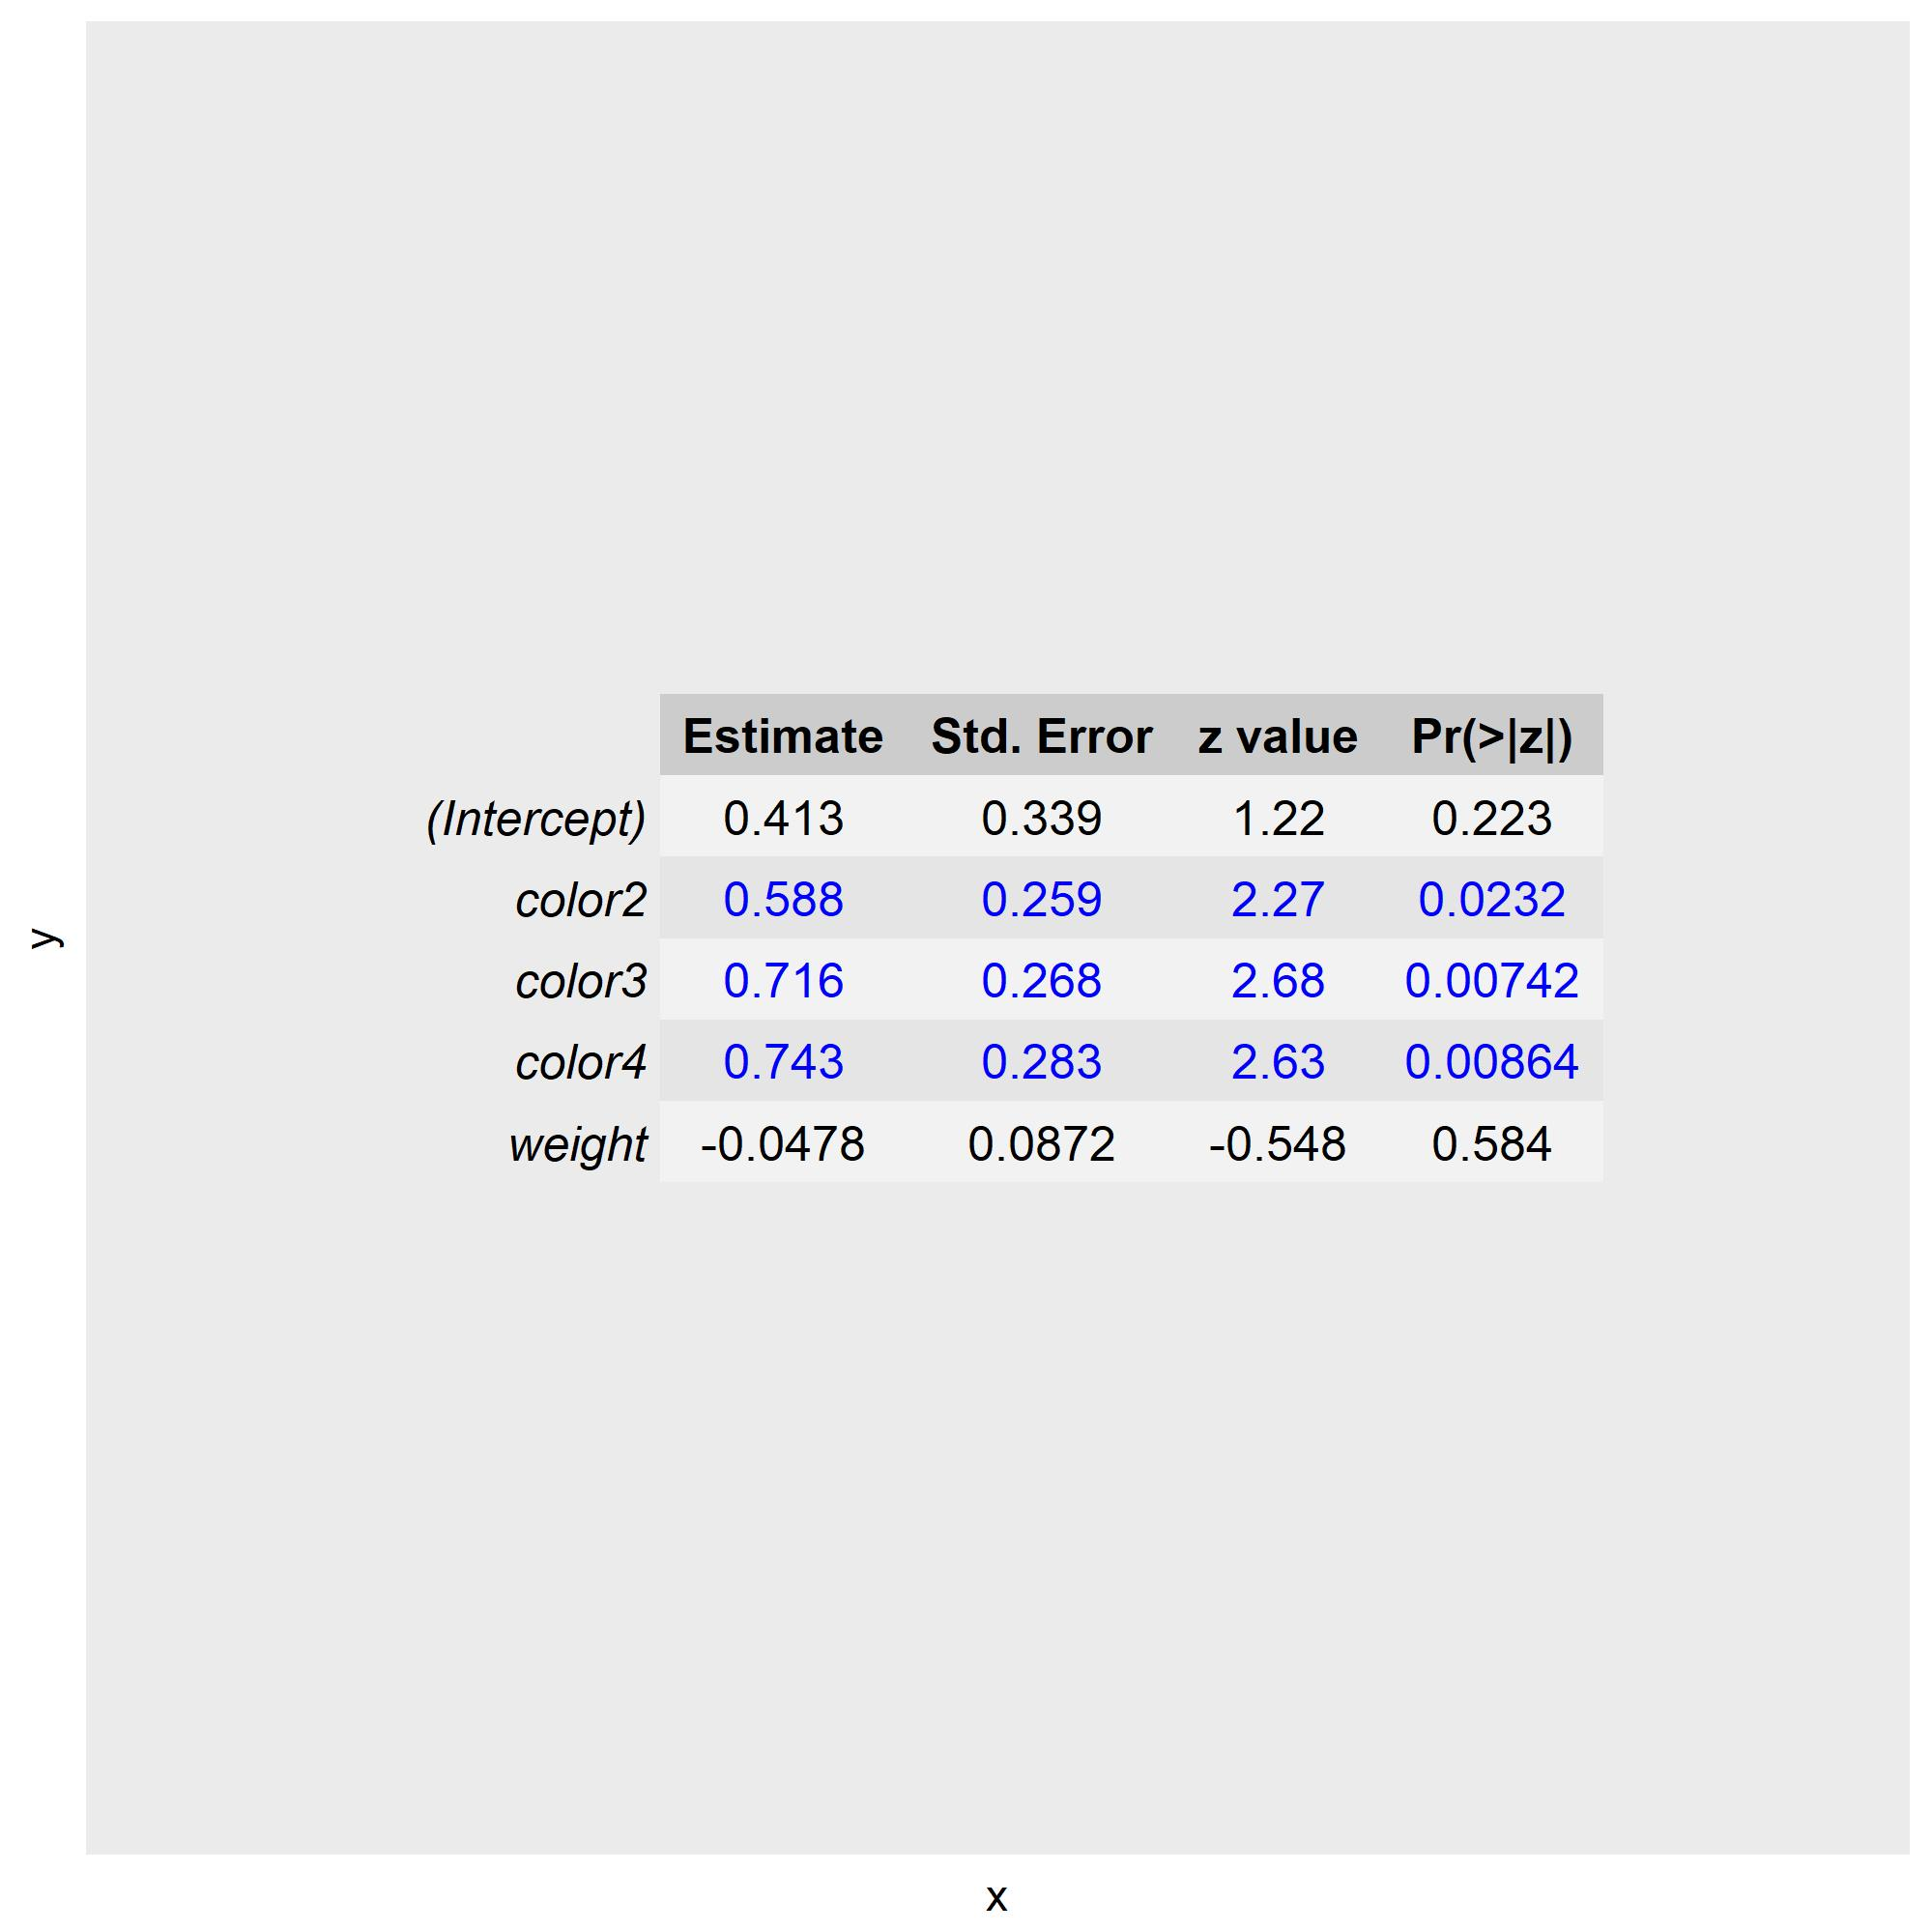
\includegraphics[scale=0.2]{poisson/poisson_color_weight} }}
    \qquad
    \subfloat[\texttt{spine = color + width}]{{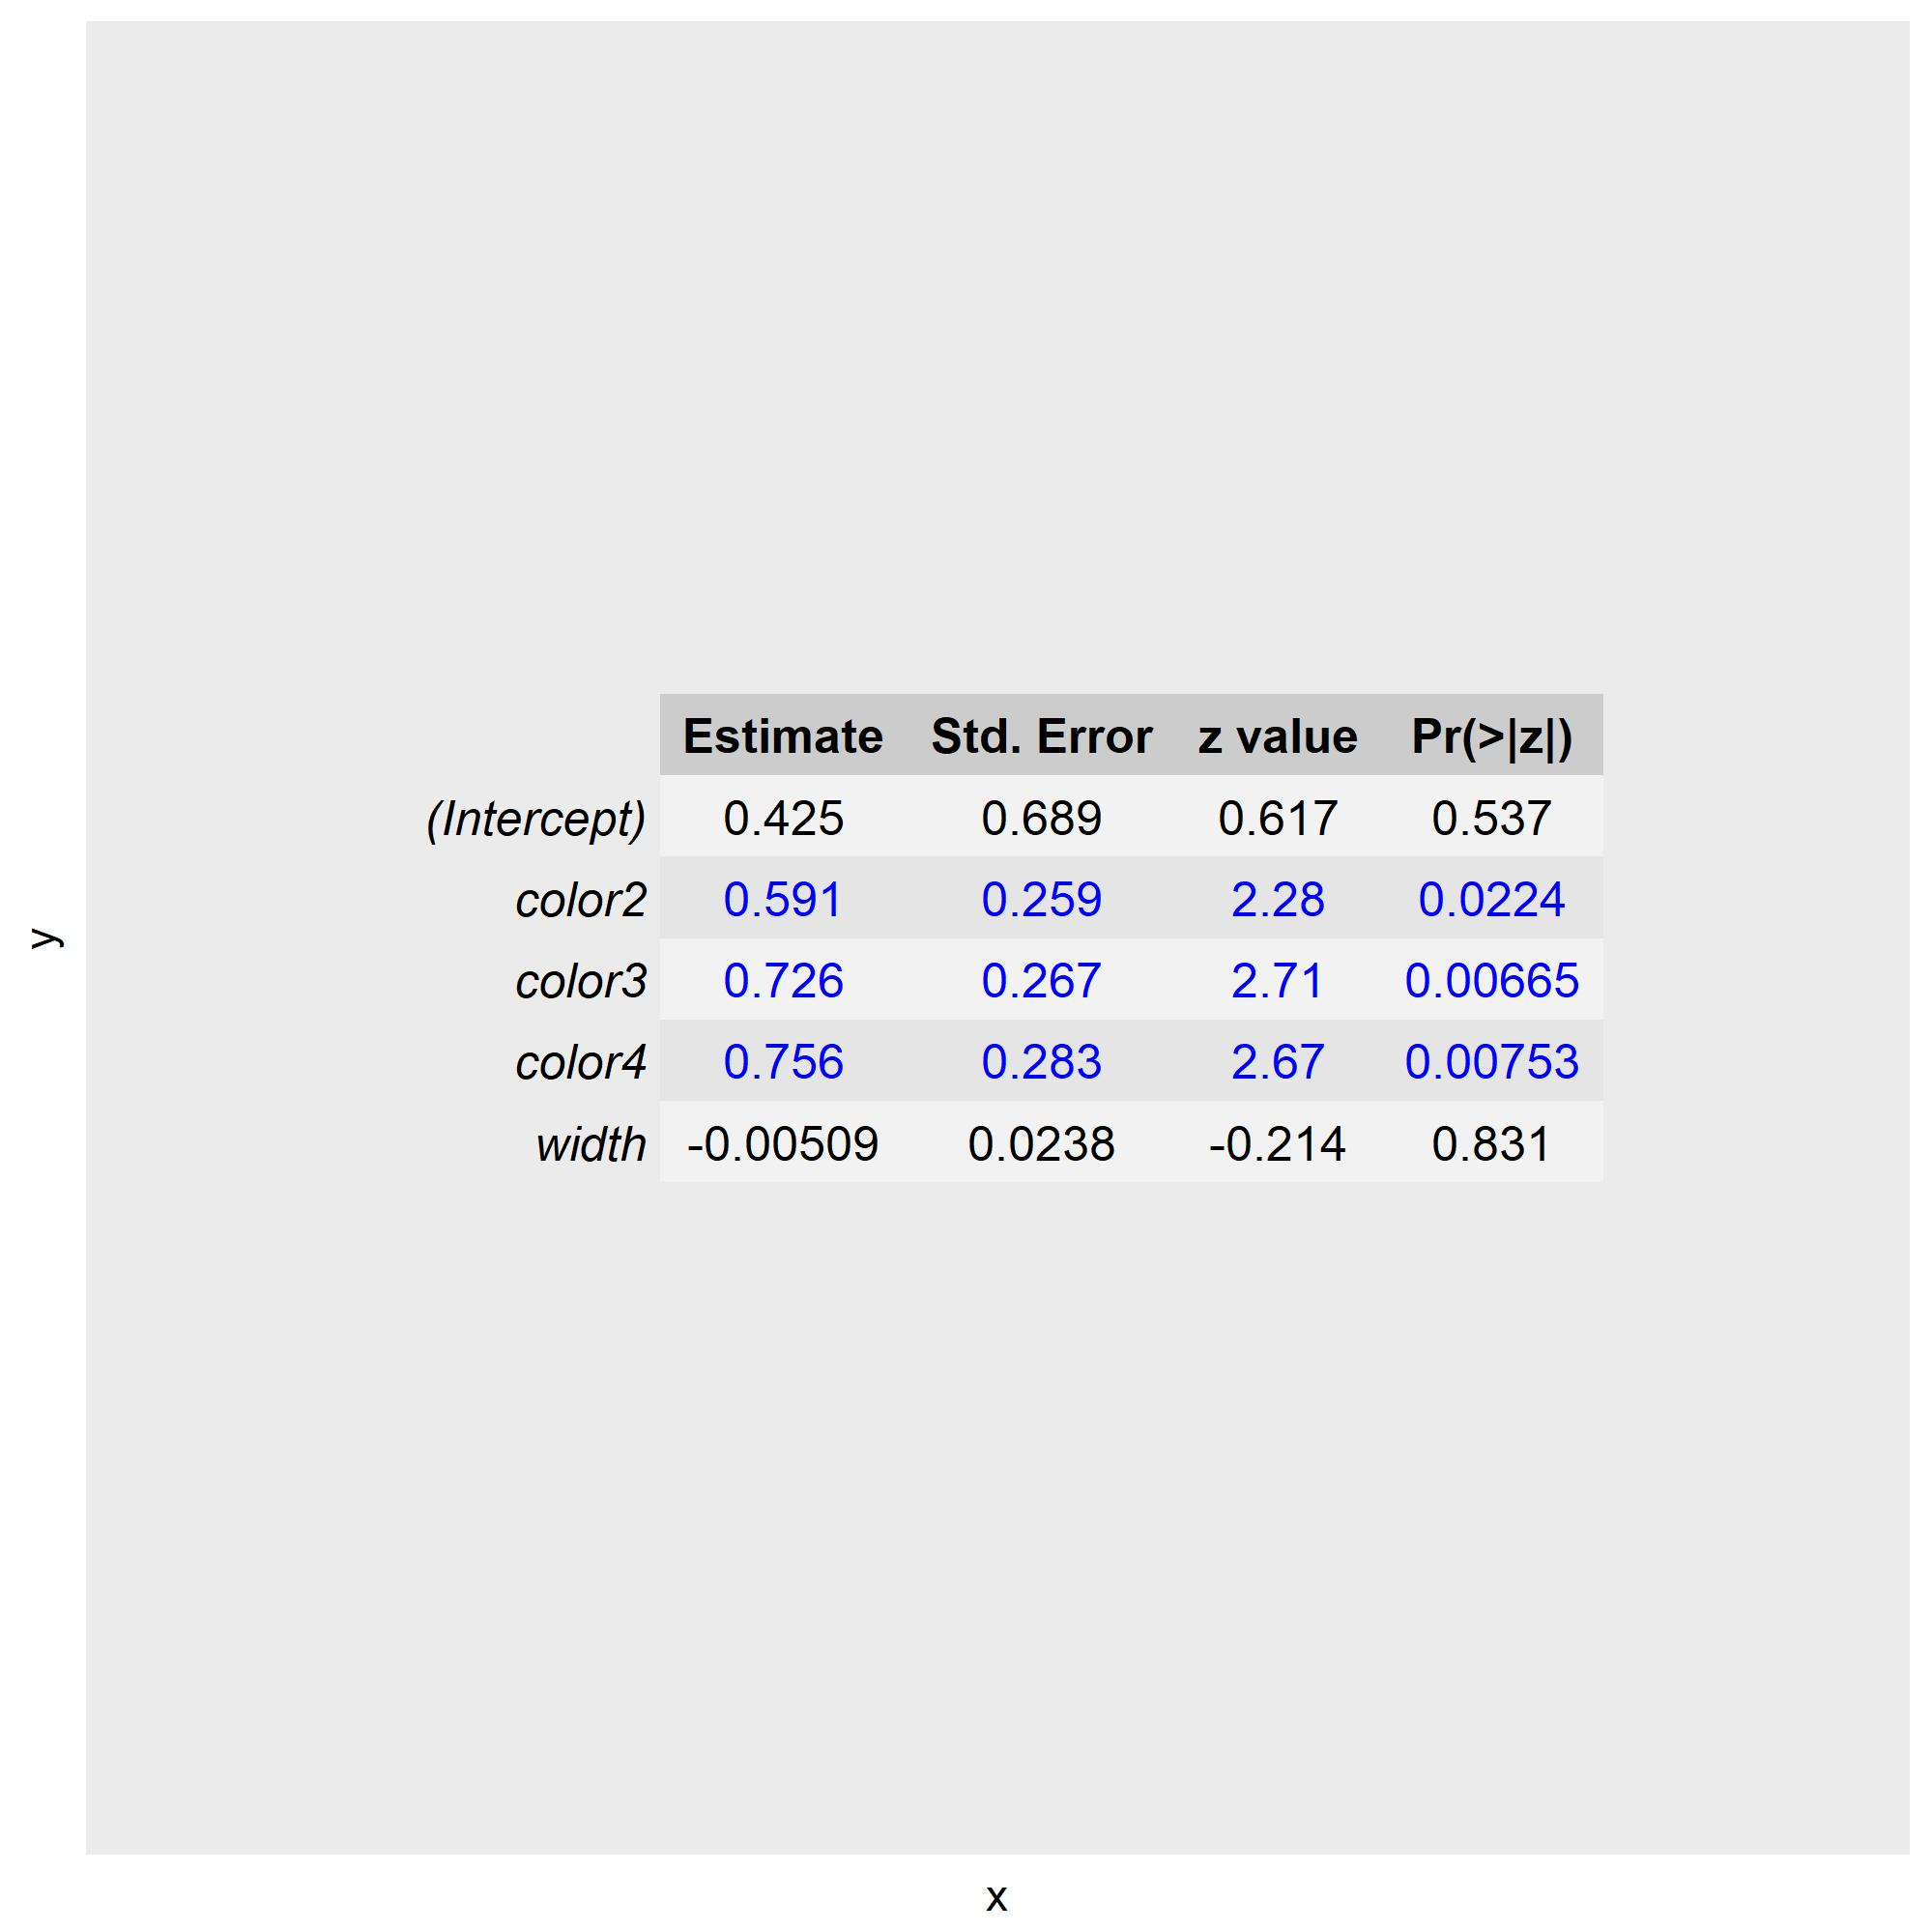
\includegraphics[scale=0.2]{poisson/poisson_color_width} }}
    \qquad
    \subfloat[\texttt{spine = color + y}]{{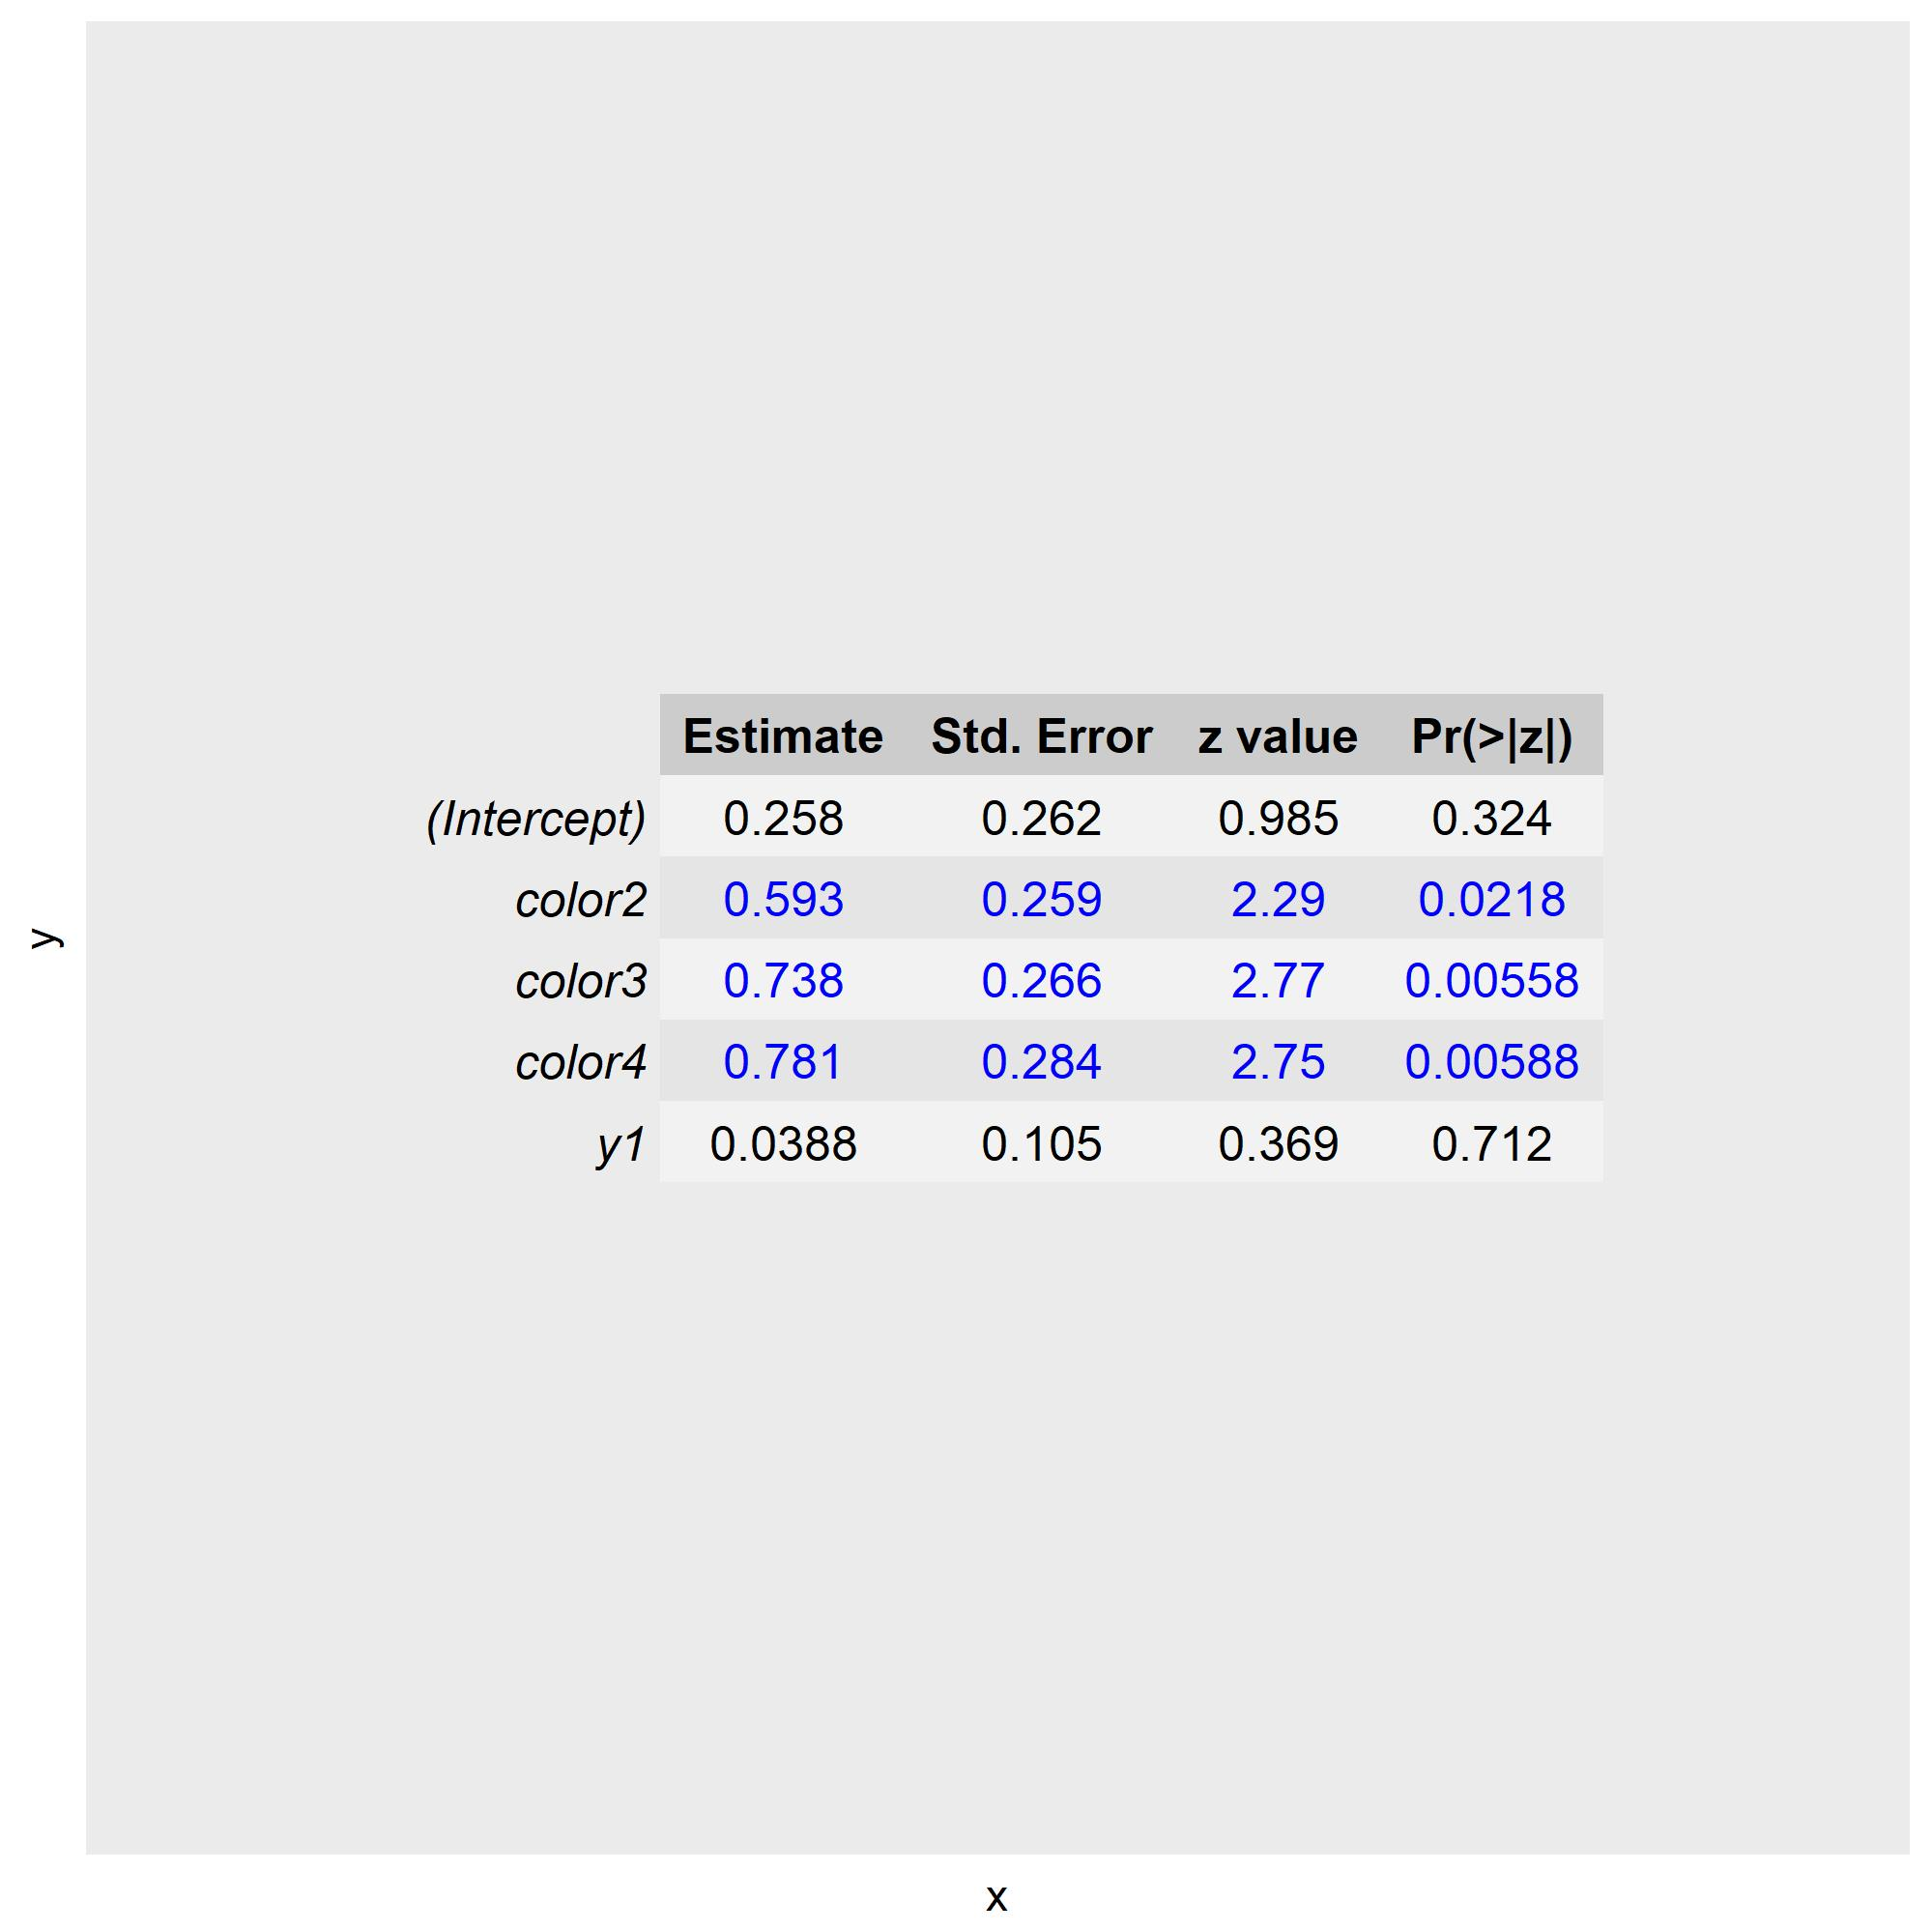
\includegraphics[scale=0.2]{poisson/poisson_color_y} }}
    \caption{Coefficients from Poisson regression models with \texttt{color} plus an additional predictor. In all four cases, the additional predictor is not significant at the 0.05 level.}
    \label{two-predictor-poisson-models}
\end{figure}

% Table generated by Excel2LaTeX from sheet 'Poisson'
\begin{table}[htbp]
  \centering
    \begin{tabular}{|c|c|c|c|c|c|c|}
    \toprule
    \multicolumn{2}{|p{13.89em}|}{Model} & \multicolumn{2}{p{8em}|}{Log-likelihood} & \multicolumn{2}{p{8em}|}{AIC} & \multicolumn{1}{c|}{\multirow{2}[4]{*}{LR test: P-value}} \\
\cmidrule{1-6}    \multicolumn{1}{|p{5.945em}|}{Reduced} & \multicolumn{1}{p{7.945em}|}{Proposed} & \multicolumn{1}{p{4em}|}{Reduced} & Proposed & \multicolumn{1}{p{4em}|}{Reduced} & \multicolumn{1}{p{4em}|}{Proposed} &  \\
    \midrule
    \multicolumn{1}{|p{5.945em}|}{spine = color} & \multicolumn{1}{p{7.945em}|}{spine = color + weight} & -260.41 & -260.26 & 528.82 & 530.52 & 0.58 \\
    spine = color & \multicolumn{1}{p{7.945em}|}{spine = color + width} & -260.41 & -260.39 & 528.82 & 530.78 & 0.83 \\
    spine = color & spine = color + sat  & -260.41 & -260.41 & 528.82 & 530.82 & 0.93 \\
    spine = color & spine = color + y  & -260.41 & -260.34 & 528.82 & 530.69 & 0.71 \\
    \bottomrule
    \end{tabular}%
    \caption*{\textbf{Table 3:} Likelihood-ratio tests and AIC values of each all models with of the form \texttt{spine = color + ?}. In all four cases, the proposed model with additional predictor fails to pass the likelihood-ratio test. Also, all proposed models have a worse AIC score compared to \texttt{spine = color}}
\end{table}%

Using a similar line of reasoning as before, likelihood ratio tests and AIC can be used to compare the reduced model \texttt{spine = color} with every other model of the form \texttt{spine = color + ?}. This is presented in Table 3, all proposed models with an additional predictor fails to pass the likelihood ratio test, and yields a worse AIC score. \\

\subsubsection{Adding interactions to the model}
\noindent At this point, it would seem difficult to improve upon  \texttt{spine = color} just by adding main effects to the model. In this study, some attempts of using models with interactions have been made. The most notable one is \texttt{spine = weight + weight:color}. The coefficients are this model are presented in Figure \ref{poisson-with-interactions}. 

\begin{figure}[H]
    \centering
    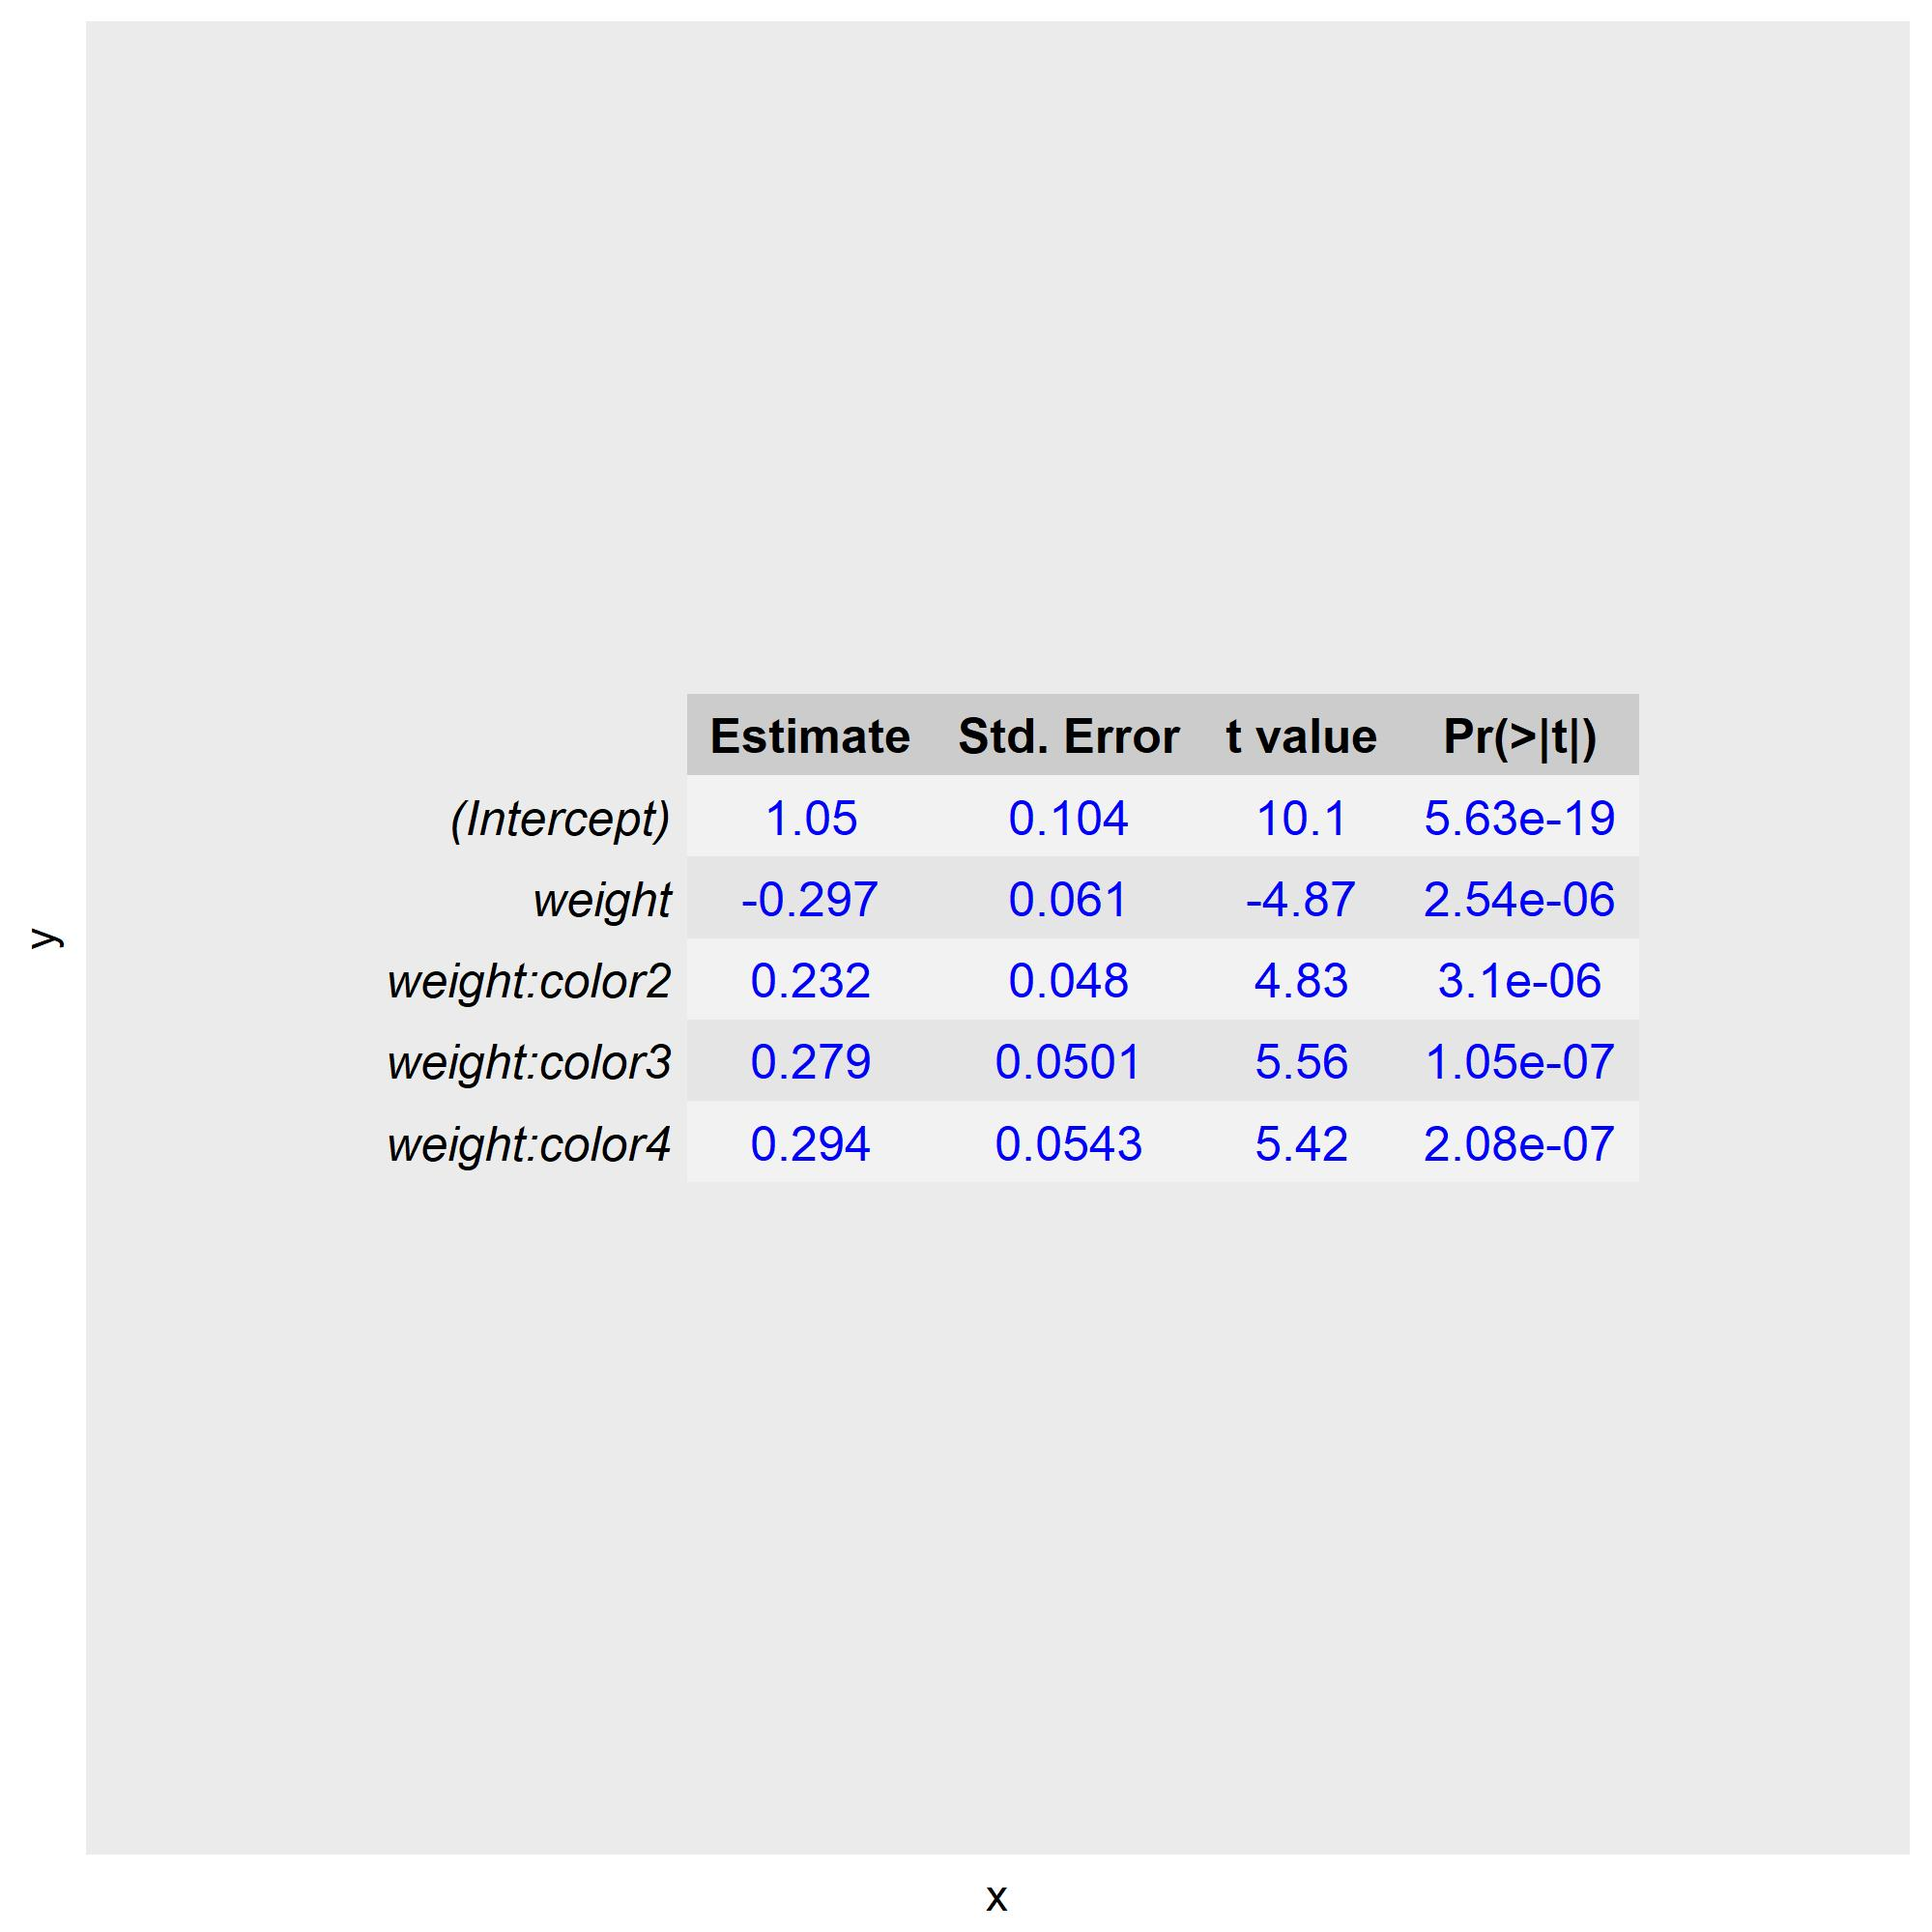
\includegraphics[scale=0.2]{poisson/poisson_weight_weightcolor} 
    \caption{Coefficients from \texttt{spine = weight + weight:color}. All predictors in the model are significant at the 0.05 level.}
    \label{poisson-with-interactions}
\end{figure}

\noindent This model has an AIC value of 530.51. The model was tested against the null model \texttt{spine = 1} and the reduced model \texttt{spine = weight} using likelihood ratio tests. In both cases, \texttt{spine = weight + weight:color} is the better model at 0.05 significance level. \\
\indent Since the predictor of \texttt{spine = color} is not present in \texttt{spine = weight + weight:color}, these two models cannot be compared using a likelihood-ratio test. In terms of AIC, \texttt{spine = color} is better (528.82). But one would wonder if \texttt{spine = weight + weight:color} would perform better in terms of predictive power, since AIC also penalizes based on the number of parameters in the model. This issue will be addressed later in Section 3.3.2. 

\subsection{Automated model selection methods}
\noindent In this section, some automated model selection techniques that was used in the study will be discussed. These methods rely heavily on R packages, and the chosen model will only be best in terms of AIC or BIC. Nonetheless, they are still very useful for identifying potentially important interactions that were not considered in manual fitting. 

\subsubsection{Stepwise selection}
The stepwise selection methods are \textit{greedy} in nature, because at each iteration, the algorithm proceeds in the direction which yields best immediate improvement (in terms of AIC). It is a computationally efficient algorithm, but does not guarantee convergence towards the optimal model. \\
\indent In this study, the \texttt{stepAIC()} function from \texttt{MASS} package was used for forward selection, backward elimination and forward-backward selection. In each case, the set of relevant predictors needs to be defined to limit the scope of models under consideration. The set of relevant predictors specified was one which includes all first, second order and third order terms, ie. all predictors within \texttt{(sat + y + weight + width + color)\textasciicircum3}. Based on this scope, models such as \texttt{spine = weight + weight:color} was also considered. \\
\indent Remarkably, all three stepwise selection techniques returns the final model \texttt{spine = color}.

\subsubsection{Exhaustive enumeration}
Exhaustive enumeration is essentially a brute force approach to the model selection problem. Under a specified set of relevant predictors, each possible combination of them are use to fit a model and compute the corresponding AIC. It is not an elegant approach, because the computational cost grows exponentially with the number of predictors. Nonetheless, the returned final model is guaranteed to be optimal from a specified scope. \\
\indent For this purpose, the \texttt{glmulti()} function from \texttt{glmulti} package \cite{calcagno_mazancourt_2010} was used. The set of relevant predictors was specified to be \textit{main effects} plus all possible pairwise interactions. The search space could not be expanded further due to limitations of the current implementation. \\
\indent The \texttt{glmulti()} function was executed twice, one with AIC as the comparison criteria, the other with BIC as the comparison criteria. In both cases, \texttt{spine = color} emerged as the optimal model.

\subsection{Additional metrics for comparison}
The analyses in section 3.2 implies that \texttt{spine = color} is indeed the best model --- in terms of AIC. But one could also argue that models such as \texttt{spine = weight + weight:color} (see figure \ref{poisson-with-interactions}) may have better predictive power due to higher complexity. In this section, alternatives to AIC and BIC that were used to compare \texttt{spine = color} with other models are presented.

\subsubsection{Pseudo R-squared}
\noindent The pseudo R-squared of a Poisson regression is defined as 
$$ R^2 = \frac{\log(\mathcal{L}(\hat{\beta_0})) - \log(\mathcal{L}(\hat{\beta}))}{\log(\mathcal{L}(\hat{\beta_0}))}$$
where $ \mathcal{L}(\hat{\beta_0}) $ is the likelihood of the null model. The pseudo R-squared of a model can be any value from 0 to 1, with 1 being a perfect fit to the dataset. Table 4 shows the pseudo R-squared values of models discussed so far. \\
\indent The two models with highest pseudo R-squared are \texttt{spine = weight + weight:color} and \texttt{spine = sat + y + weight + width + color}, this is not surprising because the pseudo R-squared is purely based on likelihood values and does not penalize the complexity of the model. One can simply include arbitrarily large number of predictors into a model to obtain a perfect pseudo R-squared of 1, but it would not be meaningful because the model has clearly overfitted on the data. 

% Table generated by Excel2LaTeX from sheet 'Poisson'
\begin{table}[H]
  \centering
    \begin{tabular}{|c|c|}
    \toprule
    \multicolumn{1}{|p{13.28em}|}{Model} & \multicolumn{1}{p{9.72em}|}{Pseudo-R-squared} \\
    \midrule
    \rowcolor[rgb]{ 1,  .922,  .612} \multicolumn{1}{|p{13.28em}|}{\textcolor[rgb]{ .612,  .341,  0}{spine = sat + y + weight + width + color }} & \textcolor[rgb]{ .612,  .341,  0}{0.206} \\
    spine = color  & 0.188 \\
    spine = weight  & 0.024 \\
    spine = width  & 0.013 \\
    spine = sat  & 0.007 \\
    spine = y  & 0.001 \\
    \multicolumn{1}{|p{13.28em}|}{spine = color + weight} & 0.193 \\
    spine = color + width & 0.189 \\
    spine = color + sat  & 0.188 \\
    spine = color + y & 0.190 \\
    \rowcolor[rgb]{ 1,  .922,  .612} \textcolor[rgb]{ .612,  .341,  0}{spine = weight + weight:color} & \textcolor[rgb]{ .612,  .341,  0}{0.194} \\
    \bottomrule
    \end{tabular}%
     \caption*{\textbf{Table 4:} The two models with highest pseudo R-squared are \texttt{spine = weight + weight:color} and \texttt{spine = sat + y + weight + width + color}, this is not surprising because the pseudo R-squared is purely based on likelihood values and does not penalize the complexity of the model (or the number of parameters of the model). It is also important to note that \texttt{spine = color} has the highest pseudo R-squared out of all single predictor models. }
\end{table}%




\subsubsection{$k$-fold cross validation error}
The $k$-fold cross validation error is an estimator of the \textit{true expected error} of a model, ie. how well a model will predict on unseen data. The algorithm to calculate this error has $k$ iterations, with the dataset being split into $k$ folds of equal size at the beginning. On the $i^{th}$ iteration, a model is fitted using all data except the $i^{th}$ fold. The fitted model is used to predict on the $i^{th}$ fold to calculate an \textit{error score}. At the end of the $k$ iterations, the average of all error scores is reported as the $k$-fold cross validation error. \\
\indent To conduct a $k$-fold cross validation, two decisions are required. The first is the choice of $k$, and the second being the definition of \textit{error function} used to measure the error between predicted value and actual value. \\
\indent Since the Horseshoe crab dataset used in this study is not large (173 records), a large value of $k$ is selected ($k = 10$) to reduce the bias of the estimate. Since the our response variable $Y$ is a count, an appropriate error function would be the widely used mean squared error, given by
$$ \text{MSE}_i = \frac{1}{n}\sum_{j=1}^{n}(y_j - \hat{y_j})^2 $$
\noindent where $\hat{y_j}$ and $y_i$ are the predicted and actual values, $n$ is the size of the $i^{th}$ fold. Table 5 shows the cross validation errors of all models experimented in section 3.1.

% Table generated by Excel2LaTeX from sheet 'Poisson'
\begin{table}[htbp]
  \centering
    \begin{tabular}{|p{14.78em}|c|c|}
    \toprule
    Model & \multicolumn{1}{p{7.61em}|}{Raw CV error} & \multicolumn{1}{p{10.335em}|}{Adjusted CV error } \\
    \midrule
    spine = sat + y + weight + width + color  & 0.600 & 0.588 \\
    \rowcolor[rgb]{ 1,  .949,  .8} spine = color  & 0.572 & 0.568 \\
    spine = weight  & 0.685 & 0.679 \\
    spine = width  & 0.696 & 0.685 \\
    spine = y & 0.693 & 0.690 \\
    spine = sat  & 0.696 & 0.686 \\
    spine = color + weight & 0.585 & 0.577 \\
    spine = color + width & 0.589 & 0.577 \\
    spine = color + sat  & 0.584 & 0.572 \\
    spine = color + y  & 0.573 & 0.571 \\
    spine = weight + weight : color & 0.585 & 0.581 \\
    \bottomrule
    \end{tabular}%
    \caption*{\textbf{Table 5:} Cross validation errors of single predictor models, models of the form \texttt{spine = color + ?}, model with all main effects, and \texttt{spine = weight + weight:color}. \texttt{spine = color} has the lowest error score, which means that it is the best model for predicting on unseen data. Judging from the errors of \texttt{spine = weight + weight:color}, we can deduce that it most probably suffers from overfitting because its higher complexity does not translate to better prediction on out-of-sample data.}
\end{table}%

\indent There is sufficient evidence to now claim that \texttt{spine = color} is indeed the best Poisson regression model for the Horseshoe crab dataset.

\subsection{Verifying model assumptions}
In this section, tools that were used to verify model assumptions of a Poisson regression model are presented. These results will help to reveal whether \texttt{spine = color} suffers from overdispersion or underdispersion.

\subsubsection{Deviance goodness of fit test}
\noindent For a Poisson regression model, the deviance statistic 
$$ D = \sum_{j=1}^{n}[y_i\log(\frac{y_i}{\exp(\beta^T{X_i})}) - (y_i - \exp(\beta^T{X_i}))] $$

\noindent is a measure of how closely the model's predictions are to the observed outcomes. If the Poisson model has $p$ parameters, $D$ would follow a chi-square distribution with $n-p$ degrees of freedom. Hence, $D$ can be used to construct a goodness-of-fit with the null hypothesis that the fitted model is correct.
In this study, the p-value returned from this hypothesis test is 1, meaning there is insufficient evidence to reject the null, which states that \texttt{spine = color} is correctly specified.

\subsubsection{Diagnostic plots}
\begin{figure}[H]
    \centering
    \subfloat[Residuals vs fitted plot of \texttt{spine = color}. The x-axis is the value of the linear predictor $\beta^TX_i$ for the $i^{th}$ data. The three curvilinear trace of points in this plot shows that response variable $Y$ is discrete and takes on three possible values. The variance in residuals appears to remain relatively constant even as $\beta^TX_i$ increases. This is a sign of underdispersion. ]{{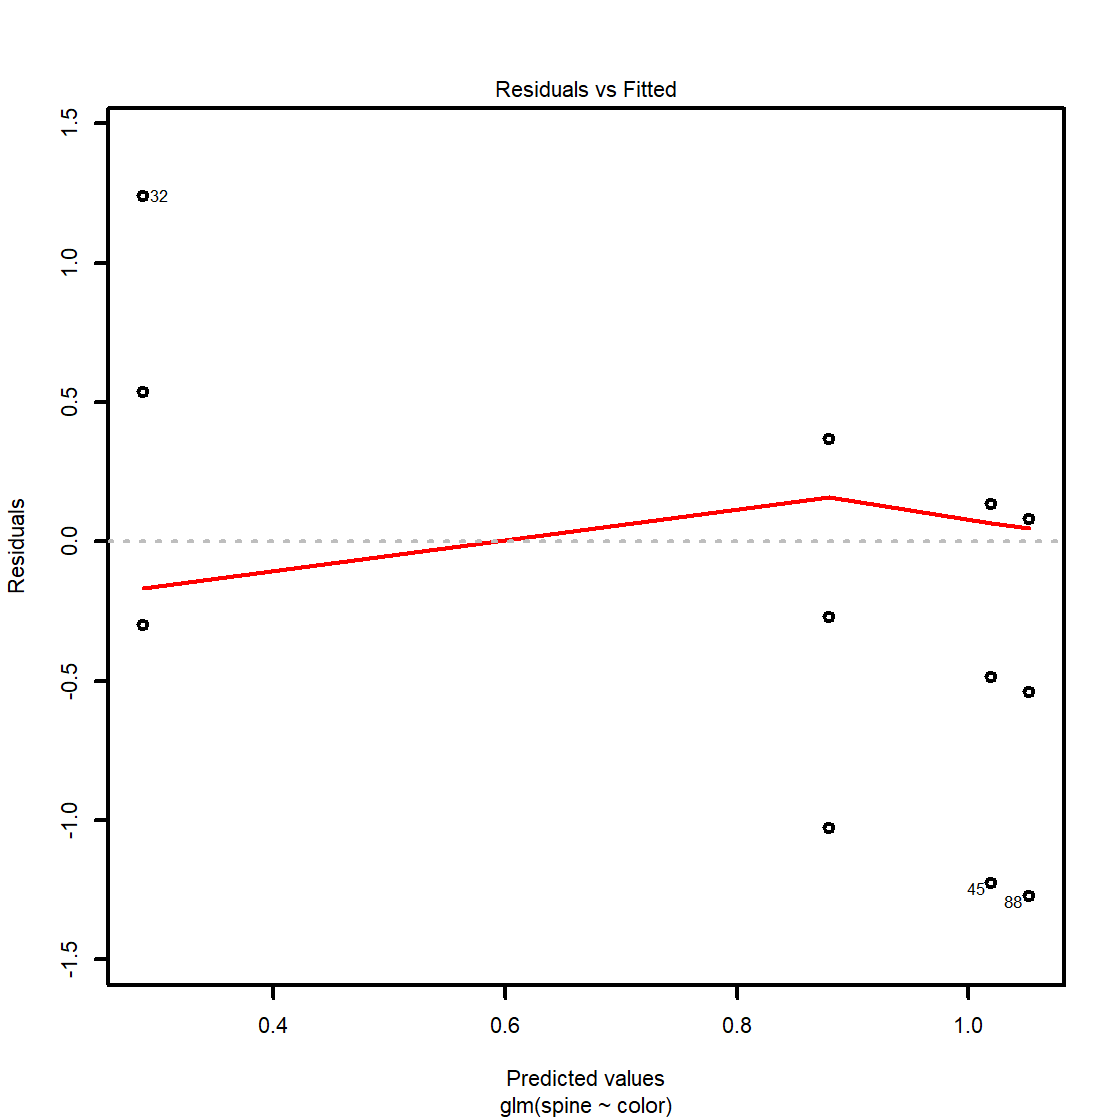
\includegraphics[scale=1.1]{poisson/poisson_color_residualsVSfitted} }}
    \qquad
    \subfloat[Standard Pearson residuals of \texttt{spine = color}. The Standard Pearson residuals corrects for the unequal variance in raw residuals by dividing the standard deviation. Based on model assumptions, it should be normally distributed with 0 mean and constant variance. However, from this plot it appears that there is a quadratic trend.]{{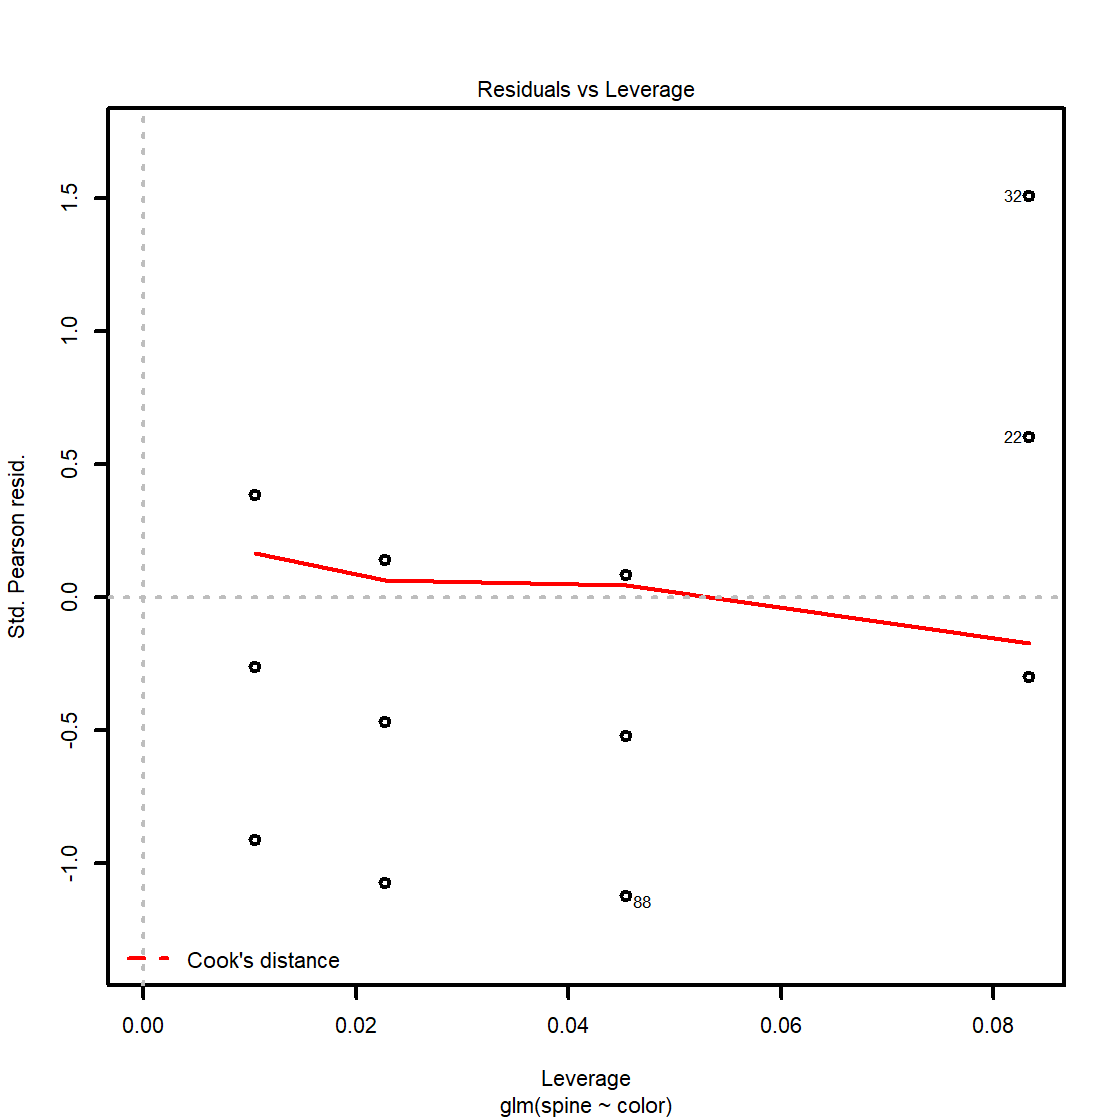
\includegraphics[scale=1.1]{poisson/poisson_color_standardpearson} }}
    \caption{Dignostic plots of \texttt{spine = color}}
    \label{disgnostic-plots}
\end{figure}

\subsubsection{Dispersion test}
\noindent Cameron and Travedi \cite{cameron_trivedi_1990} developed a test for overdispersion or underdispersion for Poisson regression models. The general framework of the hypothesis test can be described as follows:
$$ Var(Y|X) = \mu_{Y|X} + \alpha f(\mu_{Y|X})$$
$$ H_0: \alpha = 0, \quad H_1: \alpha \neq 0$$

\noindent where $\alpha \in \mathbb{R}$, $\mu_{Y|X} = E(Y|X)$, $f(\mu_{Y|X})$ is a specified monotone function (usually quadratic or linear). $H_0$ is exactly what is assumed by a Poisson model, the variance of $Y|X$ is equal to its mean. This is a two-sided test, $\alpha < 0$ means that underdispersion is occuring, while $\alpha > 0$ means that overdispersion is at work. The test statistic used is a $t$-statistic which is asymptotically standard normal under the null hypothesis. Its explicit expression is omitted here, and can be found in [reference]. \\
\indent To carry out this test on \texttt{spine = color}, the \texttt{dispersiontest()} function from \texttt{AER} package is used. This implementation supports both one-sided and two-sided versions of the dispersion test described above. The resulting p-values in Table 6 provide strong evidence that \texttt{spine = color} is suffering from underdispersion.

% Table generated by Excel2LaTeX from sheet 'Poisson'
\begin{table}[htbp]
  \centering
    \begin{tabular}{|p{5em}|p{5em}|p{6.78em}|c|c|}
    \toprule
    $H_0$    & $H_1$    & $f(\mu) = $ & \multicolumn{1}{p{9.555em}|}{Estimated value of $\alpha$} & \multicolumn{1}{p{4.78em}|}{P-value} \\
    \midrule
    \rowcolor[rgb]{ 1,  .949,  .8} $\alpha = 0$ & $\alpha \neq 0$ & $\mu$ & -0.772 & 2.20e-16 \\
    \rowcolor[rgb]{ 1,  .949,  .8}$\alpha = 0$ & $\alpha \neq 0$ & $\mu^2$ & -0.308 & 2.20e-16 \\
   $\alpha = 0$ & $\alpha > 0$ & $\mu$ & -0.772 & 1 \\
    $\alpha = 0$ & $\alpha > 0$ & $\mu^2$ & -0.308 & 1 \\
    \rowcolor[rgb]{ 1,  .949,  .8} $\alpha = 0$ & $\alpha < 0$ & $\mu$ & -0.772 & 2.20e-16 \\
    \rowcolor[rgb]{ 1,  .949,  .8} $\alpha = 0$ & $\alpha < 0$ & $\mu^2$ & -0.308 & 2.20e-16 \\
    \bottomrule
    \end{tabular}%
    \caption*{\textbf{Table 6:} Resulting p-values from the dispersion test on \texttt{spine = color}. The p-values for two-sided dispersion test, and for one-sided underdispersion test are both significant at the 0.05 level, underdispersion is clearly present in the model.  }
\end{table}%
\newpage

\section{Quasi-Poisson regression}
In section 3, \texttt{spine = color} is being identified as the best Poisson regression model for the Horseshoe crab dataset. However, it was also shown in section 3.4 that the model suffers from underdispersion. This implies that a more flexible model is required to accommodate for this behavior. The quasi-poisson regression model provides a simple solution to this problem. In a quasi-poisson model, an additional parameter $\theta$ is added into the model, such that 
$$V(Y|X) = \theta E(Y|X) = \theta \exp(\beta^TX)$$
\noindent Hence, the Poisson regression is simply a special case of quasi-poisson regression in which $\theta = 1$. $\theta$ is known as the \textbf{\textit{dispersion parameter}}. If $\theta > 1$, then the conditional variance of $Y$ increases more rapidly relative to its conditional mean, in this case the model is fitted to overdispersed data. Conversely, if $\theta < 1$, this means that the model is being fitted to an underdispersed data. If a quasi-poisson model has $k$ parameters, $\theta$ is estimated as 

$$ \hat{\theta} = \frac{1}{n-k} \sum_{j=1}^{n}{\frac{(y_i - \exp(\hat{\beta}^TX_j))^2}{\exp(\hat{\beta}^TX_j)}} $$

\noindent The estimated coefficients $\hat{\beta}$ of a model does not change when moving from a Poisson model to a quasi-Poisson model (everything else held equal). The only change is that the \textit{standard errors} of the estimated coefficients will be scaled based on the estimated value of the dispersion parameter $\theta$. This affects the statistical significance (p-values) of the estimated coefficients. \\
\indent Since the estimated coefficients remain unchanged, the estimated mean $\exp(\hat{\beta}^TX_i)$, which is used as the prediction of $y_i$, does not change. This implies that the $k$-fold Cross-Validation errors (Table 4) should remain unchanged as well when moving from a Poisson model to quasi-Poisson model. We can therefore expect \texttt{spine = color} to be the best quasi-Poisson model in terms of $k$-fold cross validation error.\\    
\indent However, the quasi-Poisson model is not a full maximum likelihood model, but a quasi-maximum likelihood model, so AIC cannot be calculated (\texttt{glm} package does not support it). This means that automated stepwise selection methods such as \texttt{stepAIC} cannot be used.

\subsection{\texttt{spine = color} with quasi-Poisson family}

\begin{figure}[H]
\begin{center}
\includegraphics[scale=0.25]{quasipoisson/poisson_color}
\caption{Coefficients of quasi-Poisson regression model \texttt{spine = color}  fitted to dataset. All predictors are significant at the 0.05 level, including the intercept. This is an improvement from the Poisson version of \texttt{spine = color} (see figure \ref{single-predictor-poisson-models}). Although the estimated coefficients remain unchanged, the standard errors associated with each coefficient is much lower. This is makes sense because it has been shown in section 3.4.3 that the Horseshoe crab dataset is underdispersed --- meaning the Poisson model for \texttt{spine = color} \textit{overestimates} the variance of the estimates of coefficients. 
}
\label{quasipoisson_color}
\end{center}
\end{figure}

Figure \ref{quasipoisson_color} shows the summary of coefficients of the quasi-Poisson model \texttt{spine = color}. As expected, the estimates of the coefficients, $\hat{\beta}$ remains the same as Poisson variant of \texttt{spine = color}. However, the p-values $\hat{\beta}$ of the quasi-Poisson model is much lower, this is a notable improvement. \\
\indent The dispersion parameter, $\hat{\theta}$ of this model was estimated to be 0.234 $(< 1)$, which is not surprising because the dataset is underdispersed. Recalling the results of one-sided underdispersion test discussed in illustrated in Table 6, the estimated value of $\alpha$, where $Var(Y|X) = \mu_{Y|X} + \alpha(\mu_{Y|X})$ was found to be -0.772. From $Var(Y|X) = \mu_{Y|X} + -0.722(\mu_{Y|X}) = 0.278\mu_{Y|X}$ which is not very far from the dispersion parameter $\hat{\theta}$ estimated by the quasi-Poisson model. This slight discrepancy is most likely due to difference in methods of estimation, the dispersion test developed by \cite{cameron_trivedi_1990} employs regression-based techniques, while the dispersion parameter $\hat{\theta}$ is simply estimated based on the Pearson statistic $$ \sum_{j=1}^{n}{\frac{(y_i - \exp(\hat{\beta}^TX_j))^2}{\exp(\hat{\beta}^TX_j)}} $$

\noindent of a Poisson model. \\
\indent Based on the results above, it is clear that the quasi-Poisson \texttt{spine = color} is a better model compared to the Poisson \texttt{spine = color}. In the next section, negative binomial regression models will be tested on the dataset.

\section{Negative Binomial regression}
The negative binomial distribution is discrete, positive-valued, and belongs to the exponential family. Thus, it fulfills equation (1) and therefore it is a feasible option for modeling the Horseshoe crab dataset. \\
\indent The negative binomial regression model is best suited for count dataset with overdispersion. This is because, in a negative binomial distribution, there is an additional dispersion parameter $\gamma > 0$ such that the variance can be written as 
$$ Var(Y) = \mu_{Y} + \frac{1}{\gamma}{\mu_{Y}}^2$$
For all $\gamma > 0$, $ Var(Y) > \mu_{Y} $, which is exactly how an overdispersed response variable $Y$ would behave. In fact, the larger $\gamma$ gets, the closer the distribution of $Y$ approximates the Poisson distribution. Formally, as $\gamma \to \infty$, we have NB($\gamma$, $\frac{\lambda}{\lambda + \gamma}$) $\to$ Poisson($\lambda$).\\
\indent Based on this reasoning, it is expected that the negative binomial model will not be a good representation of the Horseshoe crab dataset, which is underdispersed. 

\subsection{\texttt{spine = color} with negative binomial family}
The \texttt{spine = color} model was fitted using the \texttt{nb.glm} function in the \texttt{MASS} package. Figure \ref{nb_color} summarizes the estimated coefficients of the model. \\ 

\begin{figure}[H]
\begin{center}
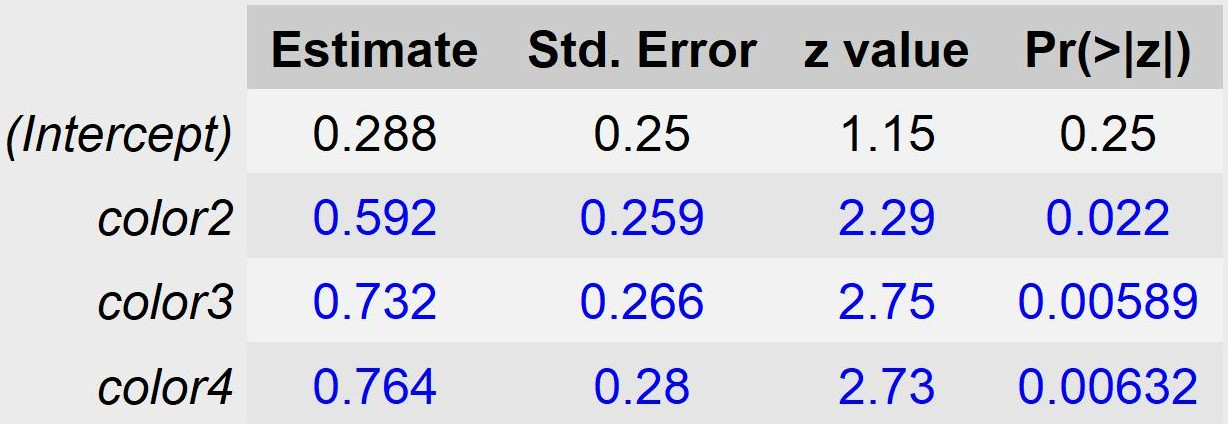
\includegraphics[scale=0.25]{nb/nb_color}
\caption{Coefficients of negative binomial \texttt{spine = color} fitted to dataset. Coefficients of \texttt{color} are significant at the 0.05 level. The model has an AIC of 530.82.}
\label{nb_color}
\end{center}
\end{figure}

The dispersion parameter was estimated to be 183942.7, a very large number. Since every negative binomial regression model is overdispersed, given an underdispersed dataset, the best possible fit would be achieved by setting $\gamma$ to be as large as possible. \\
\indent Based on this observation, it is safe to conclude that negative binomial models are not appropriate for representing the Horseshoe crab dataset.

\section{Selecting the best model}
Based on the findings from section 3, 4, and 5, it is evident that the quasi-Poisson \texttt{spine = color} is the superior model. Negative binomial regression models are inappropriate because they are not suited to model underdispersed count data, which is the case the for Horseshoe crab dataset. The quasi-Poisson \texttt{spine = color} is slightly better than the poisson \texttt{spine = color} because it accounts for the underdispersion of the Horseshoe crab dataset, which leads to more significant p-values for the estimates of ceofficients.

\section{Final adjustments: Finding outliers}
In the previous section, it is finally established that the \texttt{spine = color} quasi-Poisson model is the optimal choice among all other models, including negative binomial models and Poisson models. In this section, the goal is to examine whether there are outliers within the dataset that significantly impair the performance of the \texttt{spine = color} quasi-Poisson model.


\subsection{Cook's distance plots}
\begin{figure}[H]
    \centering
    \subfloat[]{{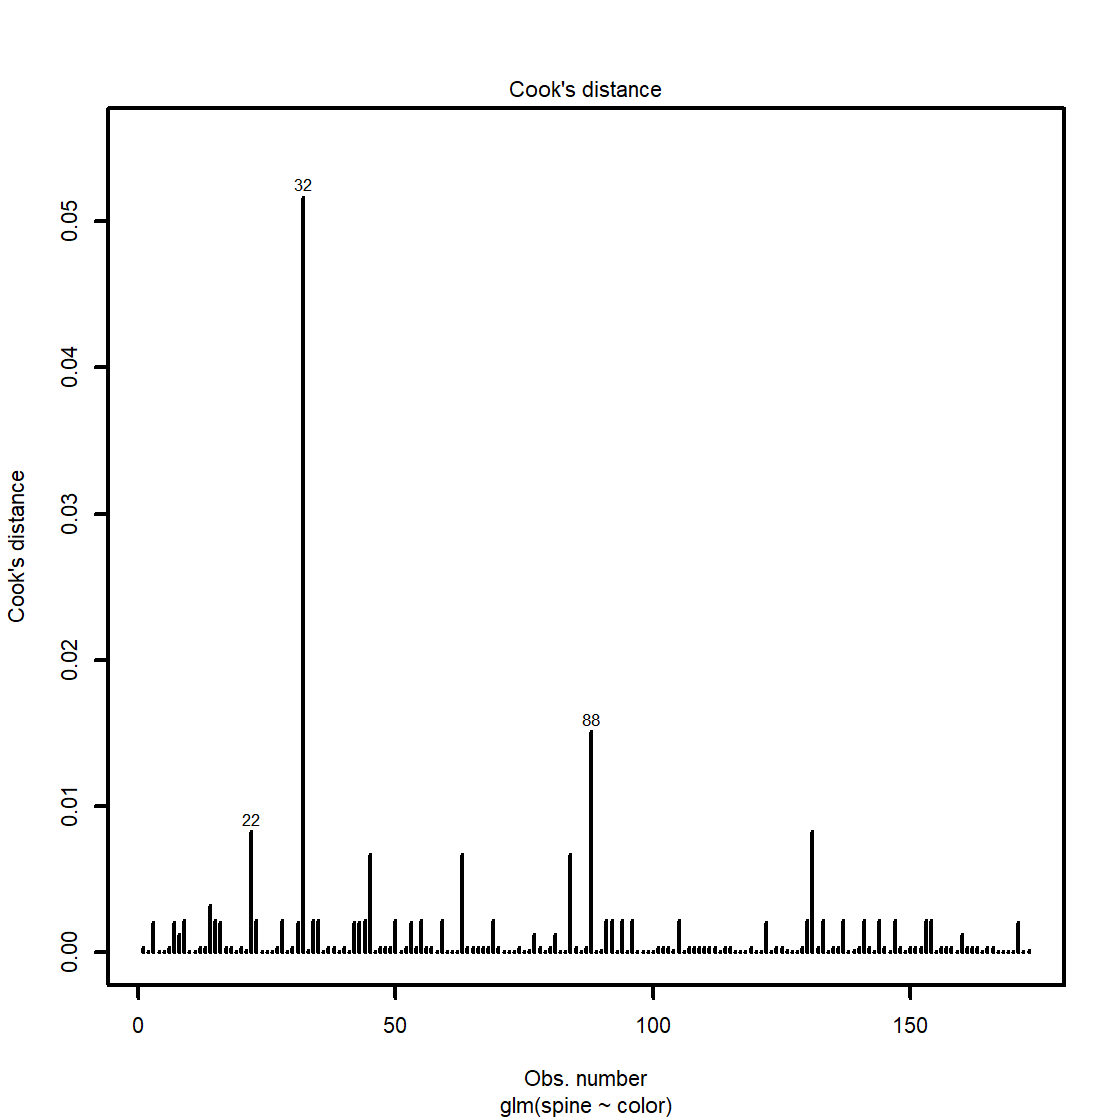
\includegraphics[scale=1.5]{poisson/poisson_color_cooksdistance} }}
    \qquad
    \subfloat[]{{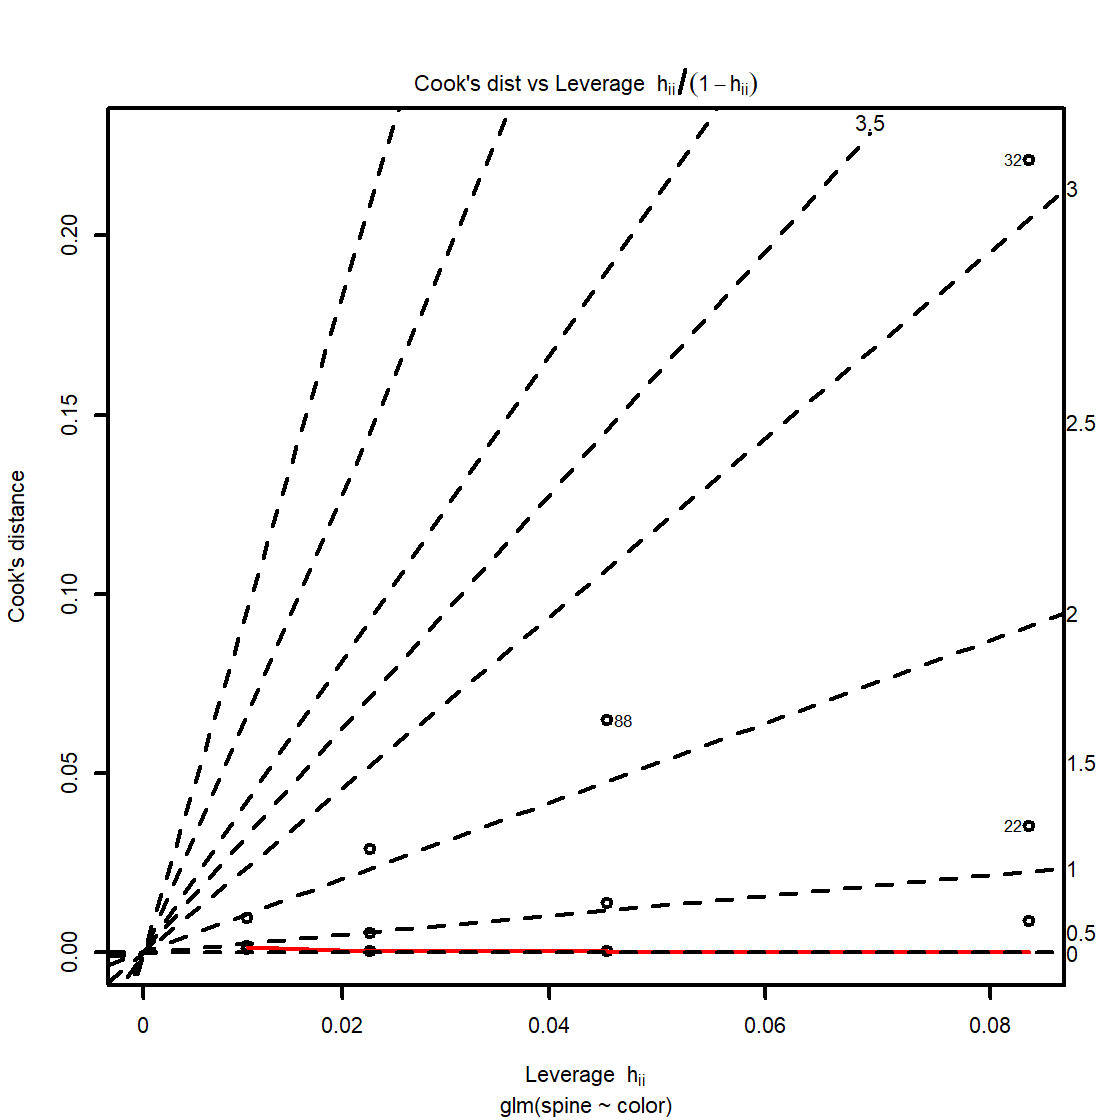
\includegraphics[scale=1.5]{quasipoisson/quasipoisson_color_cooksdistance2} }}
    \caption{Cook's distance plot of the quasi-Poisson \texttt{color = spine}}
    \label{cooks-distance}
\end{figure}


Based on the plots in figure \ref{cooks-distance}, one can easily spot the 32nd data point as a highly influential record in terms of model fitting. One of the commonly used Cook's distance threshold to decide whether a record is an outlier is $\frac{4}{N}$, where $N$ is the number of records in the dataset. Following this convention, the threshold is $\frac{4}{173} = 0.0231$. The Cook's distance of the 32nd point is at least two times this threshold, thus there is sufficient evidence to consider it as an outlier. \\
\indent Refitting the the quasi-Poisson \texttt{color = spine} without the 32nd record, we would obtain the following summary of coefficients

\begin{figure}[H]
\begin{center}
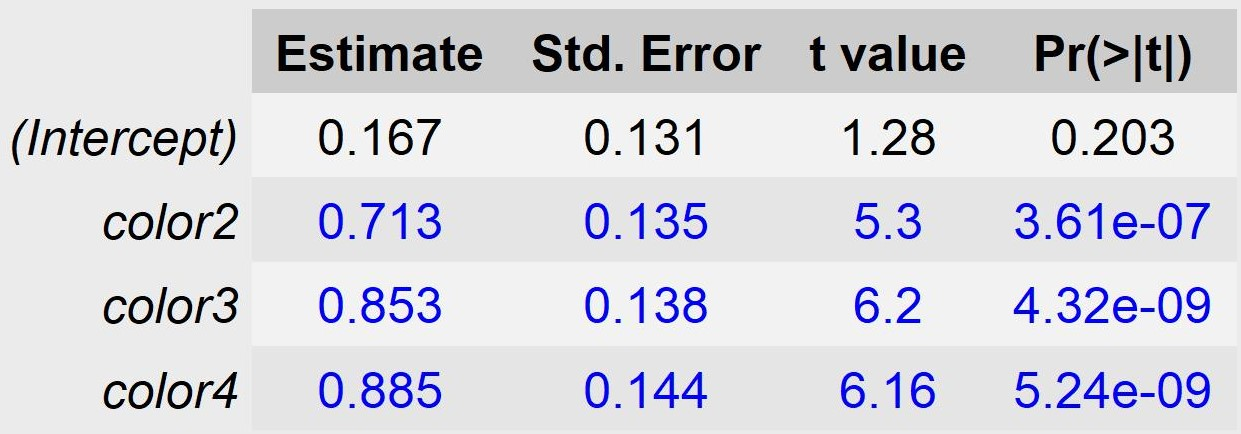
\includegraphics[scale=0.25]{quasipoisson/quasipoisson_color_without32}
\caption{Coefficients of quasi-poisson \texttt{spine = color} fitted to the dataset with 32nd record removed. It can be noted that the estimated coefficients have changed significantly compared to the previous model trained with the original dataset (see figure \ref{quasipoisson_color}).}
\label{quasipoisson_outlier_removed}
\end{center}
\end{figure}

Another way to visualize why the 32nd record is such an influential point is by simply looking at the values in this particular record. The 32nd record in the original Horseshoe crab dataset is:
\begin{itemize}
  \item \texttt{sat = 0, y = 0, weight = 2.6, width = 25.8, color = 1}
    \item \texttt{spine = 3}
\end{itemize}

Referring back to the histogram plots of \texttt{spine} with respect to \texttt{color} presented in section 2.3 (see figure \ref{distribution-of-spine-wrt-color}), we can see that there is only one record in the entire dataset where \texttt{spine} takes the value of \texttt{3} when \texttt{color} is \texttt{1}, which is precisely the 32nd record. Although similar extreme cases can also be seen when \texttt{color = 4}, the 32nd record can be expected to be much more influential on the estimated coefficient corresponding to the indicator variable of \texttt{color = 1} (ie. the intercept, see figure \ref{quasipoisson_outlier_removed}) there are only a small number of records (12) with \texttt{color = 1}.

By removing the 32nd data point, the $k$-fold Cross Validation error of the model improves significantly, decreasing from 0.572 to 0.546. The dispersion parameter $\hat{\theta}$ decreases from 0.234 to 0.223, indicating the dataset without 32nd record is slightly more underdispersed. The Cook's distance plot of this refitted model (figure \ref{quasipoisson-cooks-distance-without32}) shows that there are still several potentially influential records in the dataset, but there is no longer one specific record that stands out significantly.

\begin{figure}[H]
    \centering
    \subfloat[]{{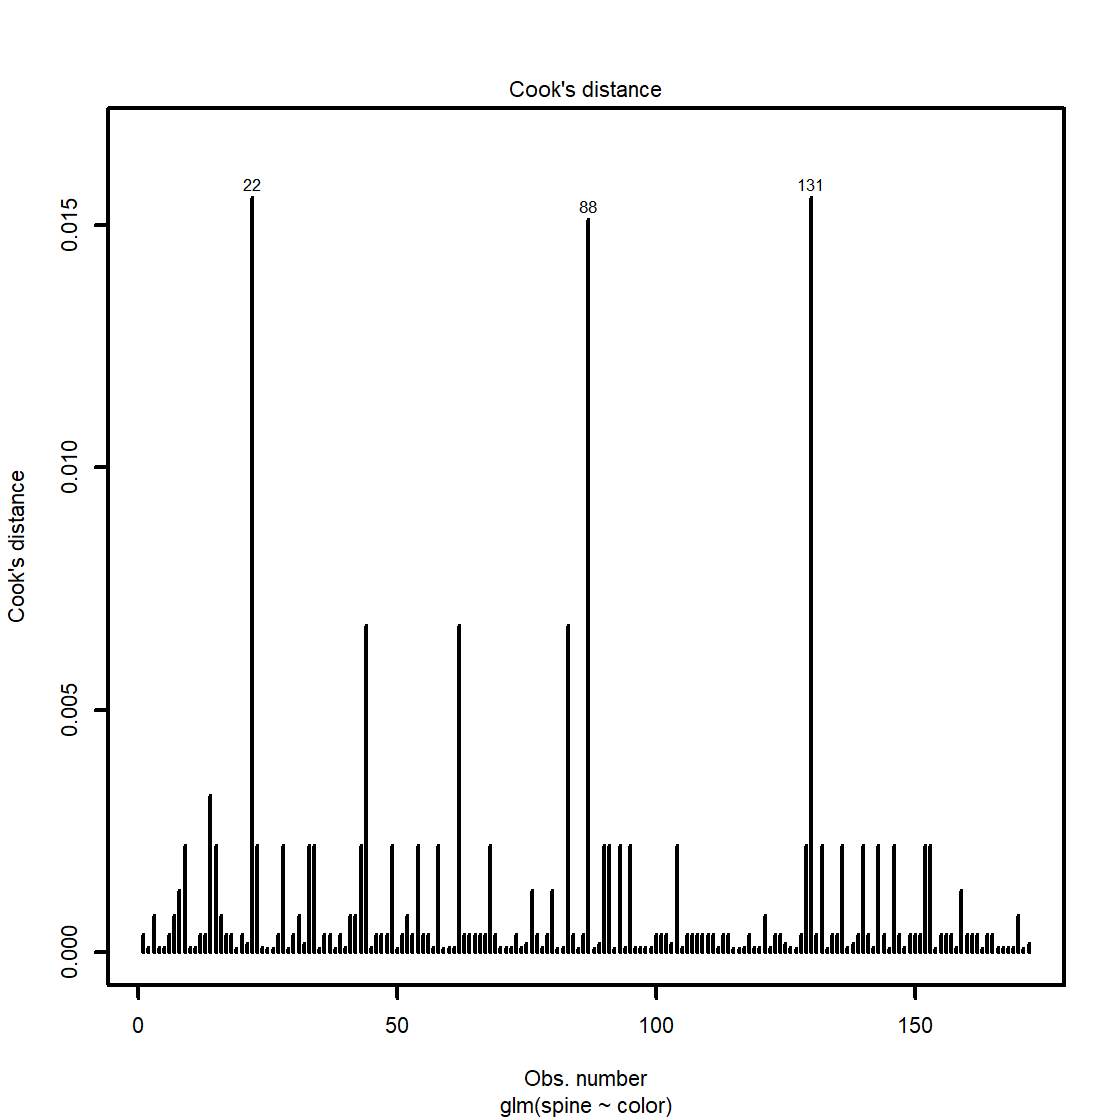
\includegraphics[scale=1.1]{quasipoisson/quasipoisson_color__without32_cooksdistance} }}
    \qquad
    \subfloat[]{{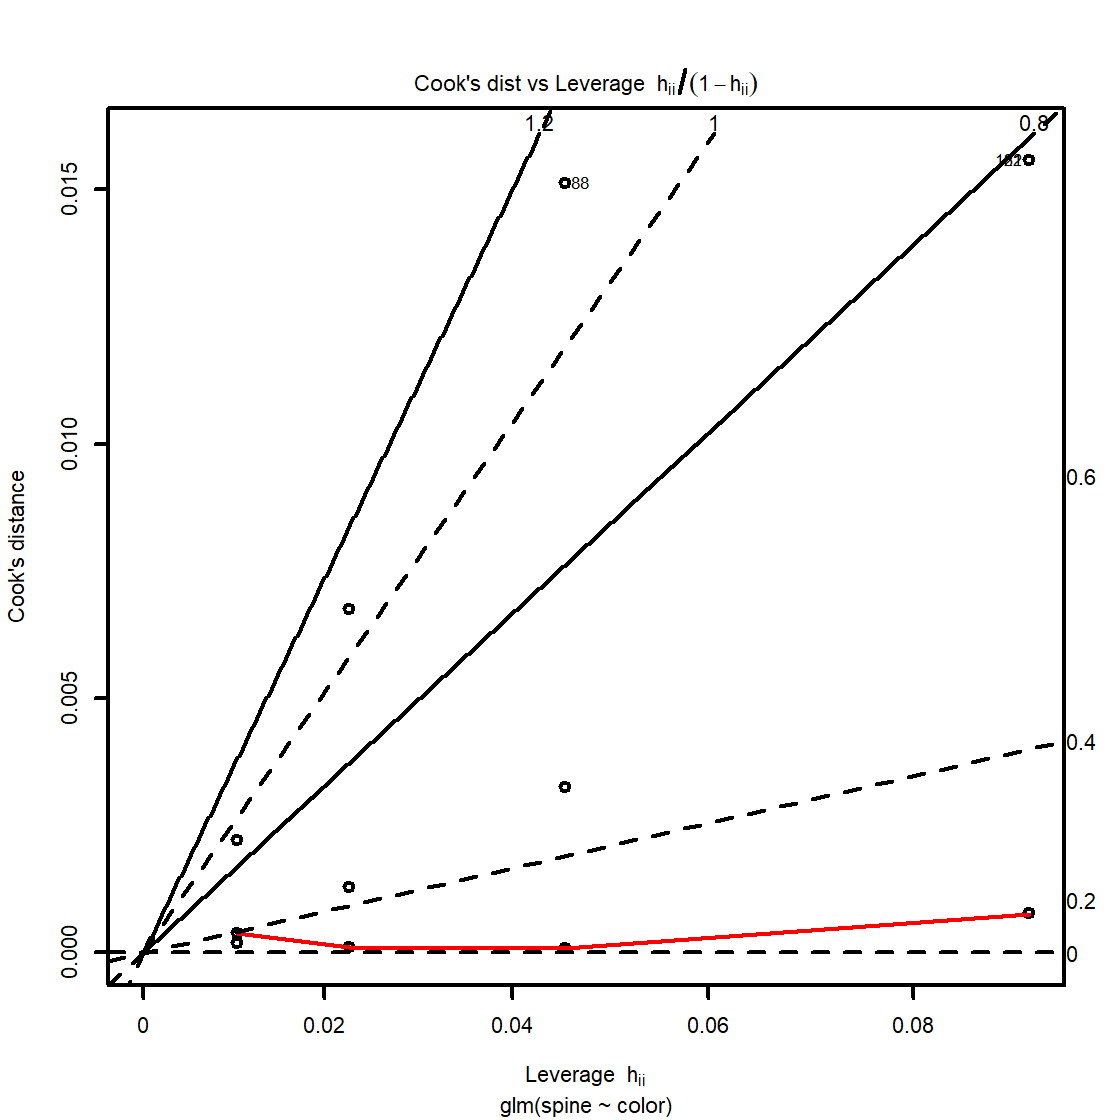
\includegraphics[scale=1.1]{quasipoisson/quasipoisson_color__without32_cooksdistance2} }}
    \caption{Cook's distance plots of the quasi-Poisson \texttt{color = spine} fitted on Horshoe crab dataset without 32nd record. There are still several potentially influential records in the dataset, but there is no longer one specific record that stands out significantly, thus this is an acceptable result.}
    \label{quasipoisson-cooks-distance-without32}
\end{figure}

\section{Conclusion}
In this study, the goal is to identify a generalized linear model that can predict \texttt{spine} in the Horseshoe crab dataset using \texttt{color, y, sat, width, weight}. Before modeling \texttt{spine}, extensive exploratory data analysis was carrierd out on dataset (section 2). Some of the visualization produced during this step proved to be extremely helpful in the latter stages of modeling. In particular, the histogram plots of \texttt{spine} with respect to \texttt{color} (see figure \ref{distribution-of-spine-wrt-color}) revealed the importance of \texttt{color} in predicting \texttt{spine}. \\
\indent A large amount of effort in this study was devoted to identifying the best possible Poisson model for predicting \texttt{spine} (section 3) before proceeding to more flexible models such as Negative Binomial models and Quasi-Poisson models. Many tools were used to compare different Poisson models, such as the AIC, BIC, likelihood ratio test, pseudo R-squared, and $k$-fold cross validation error. Automated model selection techniques was also used to efficiently explore a large set of candidate models. It was then established that \texttt{spine = color} is the best Poisson model in terms of AIC, BIC and $k$-fold cross validation error. \\
\indent Then, diagnostic plots, goodness-of-fit deviance test and dispersion test was used to verify the Poisson model assumptions. It was then discovered that the Horseshoe crab dataset is underdispersed, meaning the \texttt{spine = color} Poisson model overestimates the variance of the response variable \texttt{spine}. \\
\indent Using the valuable information gained in Poisson modeling, it was relatively easy to transition to the more flexible quasi-Poisson and Negative Binomial models. The quasi-Poisson \texttt{spine = color} was found to be a better fit to the dataset compared to the poisson \texttt{spine = color}, judging from the smaller p-values of the estimated coefficients (figure \ref{quasipoisson_color}). Negative binomial models were quickly regarded as inappropriate for this study after an experimentation because they are only suitable for modeling overdispersed count data, ie. $Var(Y|X) > E(Y|X)$.  \\
\indent Based on these results, the quasi-Poisson \texttt{spine = color} was regarded as the optimal model. Finally, in section 7, Cook's distance plots were used to identify possible outliers in the Horseshoe crab dataset. The 32nd record was removed due to its high influence on the estimated coefficients of \texttt{spine = color}.

\subsection{Future work}
Although the quasi-Poisson \texttt{spine = color} was regarded as the optimal model in this study, there are certainly many models of other distributions that can be superior. For instance, the Conway Maxwell Poisson Regression model \cite{sellers_borle_shmueli_2011} is a highly flexible regression model for count data that is able to account for underdispersion as well. In this study, the \texttt{COMPoissonReg} package in R was briefly used to explore the capabilities of the Conway Maxwell Poisson Regression. However, due to time constraint, no conclusive findings were obtained. In the future, it may be fruitful to devote time in exploring this class of models.  

\bibliographystyle{plain}
\bibliography{biblio}

\end{document} 

